\documentclass[a4paper, 11pt, oneside]{report}

\newcommand{\plogo}{\fbox{$\mathcal{PL}$}}
\usepackage{graphicx}
\usepackage{graphics}
\usepackage[utf8]{inputenc}
\usepackage{float}
\usepackage{placeins}
\usepackage[table,xcdraw]{xcolor}
\usepackage[T1]{fontenc}
\usepackage{lmodern}
\usepackage{subcaption}
\usepackage{longtable}
\usepackage[nottoc]{tocbibind}
\usepackage{url}
\usepackage{hyperref}
% \usepackage{doi}  % removed: DOIs are kept in .bib for record-keeping but not displayed in printed bibliography
\usepackage{amsmath}
\usepackage{natbib}
\usepackage[ruled,linesnumbered,vlined]{algorithm2e}
\usepackage{booktabs}
\usepackage{multirow}
\usepackage{enumitem}
\usepackage{array}
\usepackage{caption}
\usepackage{pdflscape}

\begin{document}
	\begin{titlepage}

		\centering

		\vspace*{\baselineskip}

		\vspace{0.75\baselineskip}

		{\LARGE Epileptic Seizure Detection Using Ensemble\\Machine Learning with Explainable AI}

		\vspace{0.75\baselineskip}

		\vspace{2\baselineskip}

		A report submitted for the course named Project - I (CS3201)

		\vspace*{7\baselineskip}

		Submitted By

		\vspace{0.5\baselineskip}

		{\scshape\Large Sameer Singh \\ SEMESTER - VI \\ 230101096}

		\vspace{0.5\baselineskip}

		Supervised By

		\vspace{0.5\baselineskip}

		{\scshape\Large Dr Khoirom Motilal Singh }

		\vspace{0.5\baselineskip}

		\vfill

		\begin{center}
			
\includegraphics[width=5cm]{images/iiit_manipur.png}
		\end{center}

	{\scshape\small Department of Computer Science and Engineering\\ Indian Institute of Information Technology Senapati, Manipur \\ April, 2026}

\end{titlepage}
\pagestyle{plain}

%----------------------------------------------------------------------------------------

\begin{center}
   { \LARGE \textbf{Declaration}}
\end{center}
In this submission, I have expressed my idea in my own words, and I have adequately cited and referenced any ideas or words that were taken from another source. I also declare that I adhere to all principles of academic honesty and integrity and that I have not misrepresented or falsified any ideas, data, facts, or sources in this submission. If any violation of the above is made, I understand that the institute may take disciplinary action. Such a violation may also engender disciplinary action from the sources which were not properly cited or permission not taken when needed.

\vspace{1cm}\hspace{8cm} Sameer Singh \\
\vspace{1cm}\hspace{9cm} 230101096 \\
\vspace{1cm} DATE: \underline{\hspace{4cm}}

\newpage

\begin{center}
	
\includegraphics[scale=0.2]{images/iiit_manipur.png}\\[0.2cm]
	\begin{tabular}{l}
		Department of Computer Science and Engineering \\
		Indian Institute of Information Technology Senapati, Manipur \\
	\end{tabular}
	\par\noindent\rule{\textwidth}{0.4pt}
	Khoirom Motilal Singh
	\hspace*{\fill} Email: \href{mailto:motilal@iiitmanipur.ac.in}{motilal@iiitmanipur.ac.in}\\
	Assistant Professor, CSE, IIIT Manipur
	\hspace*{0pt}\hfill Contact No: +91 70852 42211\\[1cm]
	{\Huge \textbf{\emph{To Whom It May Concern}}}\\[1cm]
	\large{This is to certify that the project report
		entitled \textbf{``Epileptic Seizure Detection Using Ensemble Machine Learning with Explainable AI'',} submitted to the department of Computer Science and Engineering, Indian Institute of Information Technology Senapati, Manipur in partial fulfilment for the award of degree of Bachelor of Technology in Computer Science and Engineering is a record of bonafide work carried out by \textbf{Sameer Singh} bearing roll number 230101096.}\\[1cm]
	\hspace*{2.6in}\large{Signature of the Supervisor}\\[0.3cm]
	\hspace*{2.5in}\textbf{(Khoirom Motilal Singh)}\\[0.6cm]
\end{center}

\noindent Signature of the Examiner 1 ............................\\[0.5cm]
\noindent Signature of the Examiner 2 ............................\\[0.5cm]
\noindent Signature of the Examiner 3 ............................\\[0.5cm]
\noindent Signature of the Examiner 4 ............................

\newpage
\begin{center}
    {\LARGE \textbf{Abstract}}
\end{center}
\vspace{0.5cm}

\textbf{Epileptic seizure detection} from electroencephalogram (EEG) signals is a challenging problem in biomedical signal processing. Manual inspection of EEG recordings is time-consuming, subjective, and constrained by the availability of trained neurologists. Automated machine learning approaches offer a reliable alternative, but most existing systems rely on narrow feature sets, single classifiers, and provide no transparency in their decisions.

This project introduces \textbf{EpiDetect}, an automated seizure detection pipeline built on the publicly available Bonn University EEG dataset~\citep{andrzejak2001indications}. Raw single-channel signals are preprocessed using a fourth-order Butterworth bandpass filter (0.5--85~Hz) and z-score normalization. Each signal is divided into 16 equal segments, from which \textbf{720 features} are extracted across four complementary domains: discrete wavelet transform coefficients (Daubechies-4, four levels), time-domain statistics including Hjorth parameters and Teager energy, frequency-domain band powers, and nonlinear complexity measures such as sample entropy, permutation entropy, detrended fluctuation analysis, and Higuchi fractal dimension. A union-based \textbf{feature selection} strategy combining mutual information and ANOVA F-classification retains the most discriminative subset.

Classification is performed by a \textbf{soft-voting ensemble} of eight diverse classifiers, namely Random Forest, Extra Trees, Histogram Gradient Boosting, Support Vector Machine, Multilayer Perceptron, Gradient Boosting, AdaBoost, and K-Nearest Neighbours, trained with five random seeds to stabilize predictions. Under \textbf{10-fold stratified cross-validation}, the system achieves 99.40\% accuracy, 98.00\% recall, and 99.92\% AUC-ROC, with only three misclassifications out of 500 signals. \textbf{SHAP-based explainability} is integrated to make every prediction transparent, producing global feature importance rankings, beeswarm summary plots, and permutation importance analysis. The pipeline is served through a Flask REST API with a web dashboard for signal upload, prediction display, and explanation inspection.

\pagebreak

        \begin{center}
            { \LARGE \textbf{Acknowledgement}}
        \end{center}
	\vspace{2cm}

I am grateful to my project supervisor, \textbf{Dr.~Khoirom Motilal Singh}, Assistant Professor, Department of Computer Science and Engineering, IIIT Senapati, Manipur, for his constant guidance, constructive feedback, and encouragement throughout the development of this project. His direction was instrumental in shaping the methodology and ensuring the rigour of the work.

I wish to acknowledge \textbf{Andrzejak et al.} for making the Bonn University EEG dataset publicly available, which formed the experimental foundation of this project. I am also thankful to \textbf{Chanu et al.} and \textbf{Chen et al.} for their published work, which informed several design decisions in this project.

I would also like to thank my peers and classmates for their valuable discussions and insights, which helped refine my understanding at various stages of this work.

	\vspace{1cm}

	\hspace{9cm}Sameer Singh\\
	\hspace{9cm}230101096

	\newpage
	\tableofcontents
	\listoffigures
        \listoftables
	\chapter{Introduction}
	
\section{Background}

Epilepsy ranks among the most common long-term neurological conditions worldwide. The World Health Organization estimates that roughly 50 million people live with epilepsy globally, spanning all age groups, geographies, and socioeconomic backgrounds~\citep{who2019epilepsy, chanu2023automated}. The disorder manifests through recurrent seizures, which are brief episodes of involuntary movement, altered consciousness, or unusual sensations triggered by sudden, synchronized bursts of abnormal electrical activity in the brain. What makes epilepsy especially dangerous is its unpredictability; a seizure can occur while a person is cooking, crossing a road, or sleeping.

The electroencephalogram (EEG) has been the workhorse of epilepsy diagnosis for decades. Thin electrodes placed on the scalp pick up the electrical signals generated by large populations of neurons, tracing them as oscillating waveforms over time. A trained neurologist can distinguish the high-amplitude, chaotic spikes of a seizure from the relatively calm rhythms of healthy brain activity. But this visual inspection is far from straightforward. A routine clinical EEG recording might run for half an hour; continuous monitoring in intensive care can stretch to several days. Scanning through all that data to spot episodes that may last only a few seconds demands considerable time, focus, and expertise~\citep{adeli2003analysis}.

\section{Problem Statement}

The manual review of EEG recordings for seizure detection suffers from several well-documented problems. First, it is extremely labour-intensive. A neurologist must carefully examine hours of waveform data to locate brief seizure events that can easily be missed during a lapse in attention. Second, the process is inherently subjective. Two experienced clinicians may look at the same stretch of EEG and arrive at different conclusions, especially for borderline or ambiguous patterns~\citep{chanu2023automated}. Third, there is a global shortage of trained EEG specialists, particularly in rural clinics and low-resource settings, leading to long waiting times and delayed diagnoses.

These challenges have motivated researchers to explore automated approaches. Over the past decade, a range of machine learning methods have been proposed to assist clinicians by flagging potential seizure events in EEG data. However, many of these systems share one or more of the following weaknesses:

\begin{enumerate}[leftmargin=2cm]
    \item They extract features from only one or two signal analysis domains (typically wavelets alone), overlooking complementary information that other domains could contribute.
    \item They depend on a single classifier, which may not generalize well across different patient populations or recording conditions.
    \item They offer no form of interpretability; the model outputs a decision but provides no explanation for why it arrived at that conclusion. In clinical settings, this opacity erodes trust and limits practical adoption.
\end{enumerate}

\section{Motivation}

Two observations drive this project. The first is that most existing seizure detection systems operate as black boxes. A physician receives a verdict, either ``seizure detected'' or ``normal'', without any insight into the signal characteristics that led to that judgement. In a medical context, where the stakes are high and accountability matters, this is a serious limitation. Clinicians want to see the evidence, not just the conclusion.

The second observation is that the feature engineering in prior works is often narrow. Chanu et al.~\citep{chanu2023automated} showed that discrete wavelet transform (DWT) features paired with an optimized neural network can reach 99.2\% accuracy on the Bonn dataset. Chen et al.~\citep{chen2023epileptic} demonstrated that combining DWT-based entropy features with a Random Forest selector and a CNN classifier can achieve high accuracy across multiple binary classification tasks on the same dataset. Both studies confirmed the usefulness of wavelet-based analysis, but neither explored a broad, multi-domain feature set, and neither integrated any form of post-hoc explainability.

This project builds on those ideas in three specific ways:

\begin{itemize}
    \item It extracts a much larger feature set of 720 features spanning four different analysis domains, namely wavelet, time, frequency, and nonlinear, capturing a wider range of the signal's behaviour.
    \item It replaces single-model classification with an ensemble of eight distinct classifiers combined through soft voting and multi-seed averaging, improving both accuracy and stability.
    \item It integrates SHAP-based explanations into every prediction, so that each output comes with a transparent account of which features contributed to it and by how much.
\end{itemize}

\section{Objectives}

The key objectives of this project are:

\begin{enumerate}[leftmargin=2cm]
    \item To preprocess raw EEG recordings from the Bonn University dataset using a fourth-order Butterworth bandpass filter (0.5--85~Hz) and z-score normalization.
    \item To engineer a comprehensive set of 720 features from each signal, covering discrete wavelet transform coefficients, time-domain statistics, frequency-domain band powers, and nonlinear complexity measures.
    \item To apply a union-based feature selection strategy combining mutual information and ANOVA F-classification scores, retaining only the most discriminative features.
    \item To train a soft-voting ensemble of eight classifiers, namely Random Forest, Extra Trees, Histogram Gradient Boosting, SVM, MLP, Gradient Boosting, AdaBoost, and KNN, and evaluate it through 10-fold stratified cross-validation.
    \item To integrate SHAP (SHapley Additive exPlanations) for model transparency, producing global feature importance rankings, SHAP summary plots, and permutation importance analysis.
    \item To deploy the trained pipeline as a Flask-based REST API backed by a web dashboard where users can upload EEG files, view predictions, and inspect explanations.
\end{enumerate}

\section{Scope of the Project}

This project is scoped to the Bonn University EEG dataset, which contains 500 single-channel recordings distributed across five clinical categories. The classification task is binary: seizure (Set~E) versus non-seizure (Sets~A through~D). The system is designed as a proof-of-concept demonstrating that ensemble learning combined with explainable AI can deliver both high accuracy and clinical transparency. It does not aim to replace the judgement of a neurologist; rather, it is intended to serve as an assistive screening tool that can speed up initial triage.

\section{Project Timeline}

Development was carried out over four months, from January to April 2026, organized into six overlapping phases. Figure~\ref{fig:timeline} presents the schedule.

\begin{figure}[H]
\centering
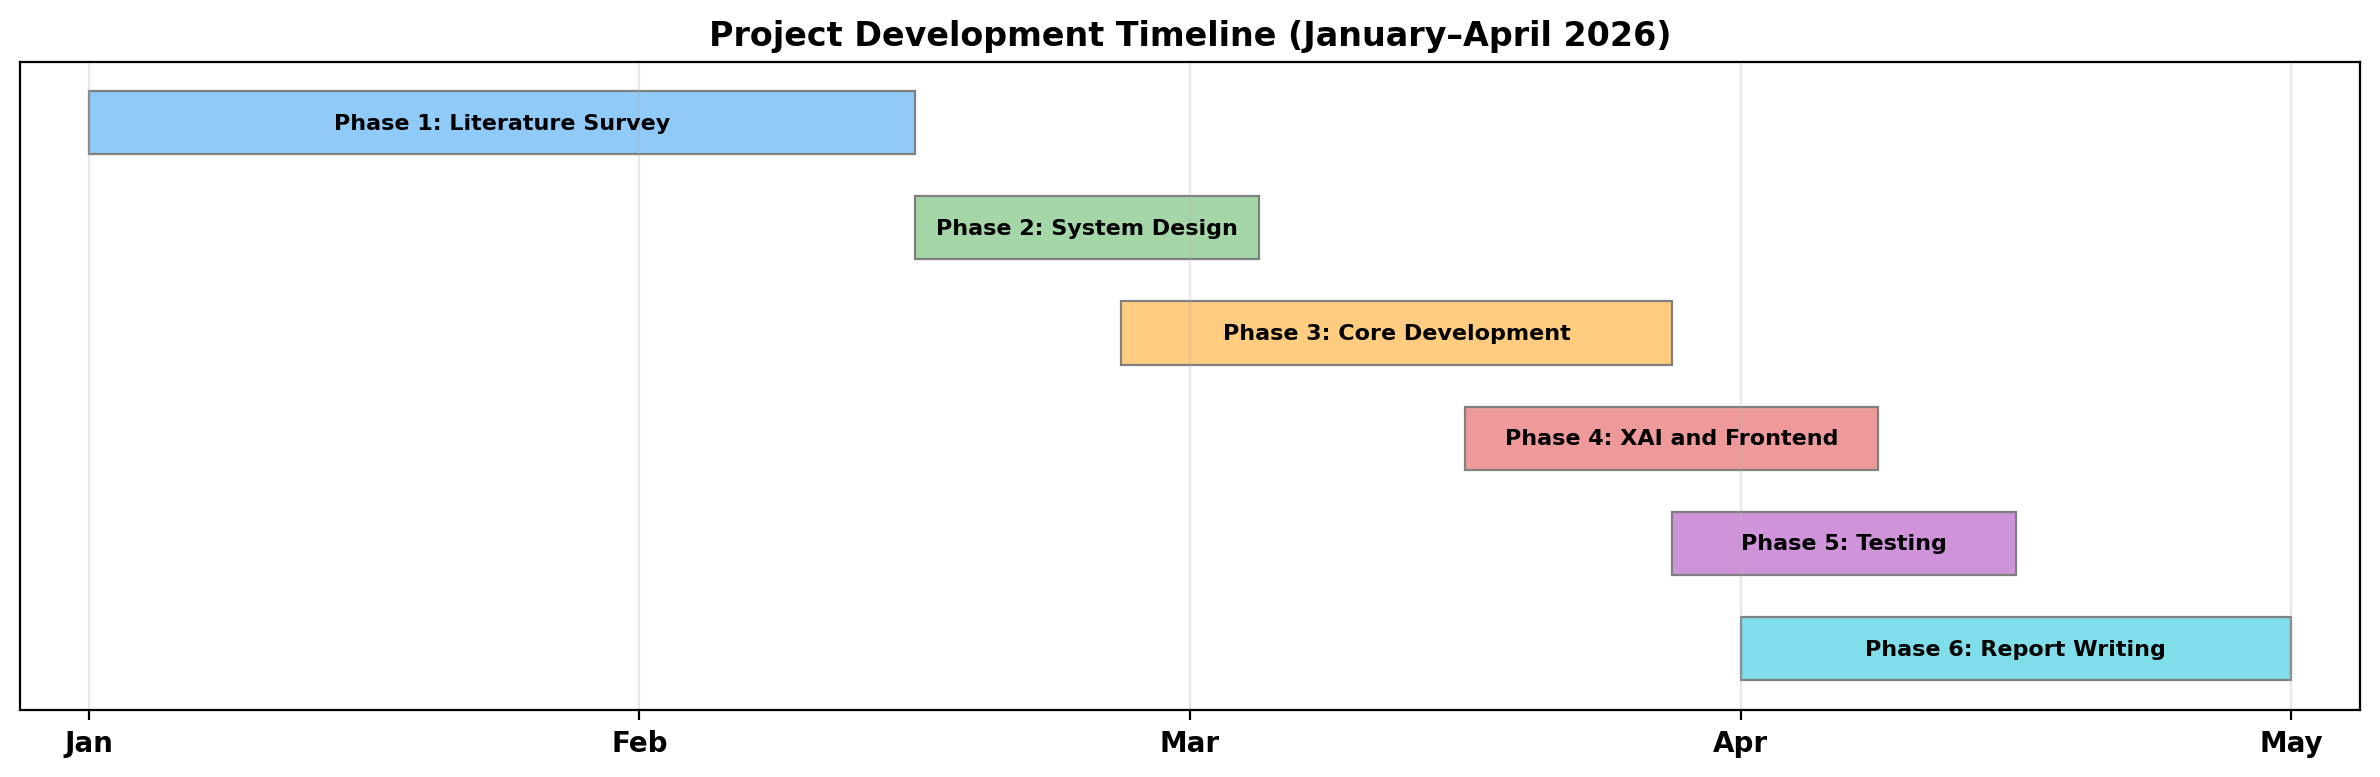
\includegraphics[width=\textwidth]{images/gantt_chart.png}
\caption{Project development timeline (January--April 2026).}
\label{fig:timeline}
\end{figure}

\begin{itemize}
    \item \textbf{Phase~1 (January--mid February):} Studying existing seizure detection methods, reading the base papers by Chanu et al. and Chen et al., understanding the Bonn dataset, and identifying gaps in current approaches.
    
    \item \textbf{Phase~2 (mid February--late February):} Deciding on the modular pipeline architecture, choosing the feature domains and classifiers, and setting up the project directory structure.
    
    \item \textbf{Phase~3 (late February--mid March):} Implementing the data loader, signal preprocessing module, multi-domain feature extraction (720 features), and the eight-classifier ensemble with multi-seed training.
    
    \item \textbf{Phase~4 (mid March--late March):} Adding SHAP-based explainability, building the Flask REST API, and developing the frontend dashboard with EEG visualization.
    
    \item \textbf{Phase~5 (late March):} End-to-end testing, debugging, validating metrics under cross-validation, and ensuring the API and frontend work correctly together.
    
    \item \textbf{Phase~6 (April):} Writing the project report, compiling results, generating figures and tables, and preparing the final submission.
\end{itemize}

\section{Organization of the Report}

The remainder of this report is laid out as follows. Chapter~2 surveys existing literature on automated seizure detection, discussing the strengths and shortcomings of earlier methods. Chapter~3 covers requirements engineering, including feasibility analysis, use case modelling, and the software requirement specification. Chapter~4 describes the system design with architecture diagrams, data flow, and module-level design. Chapter~5 presents the implementation in detail, along with formal algorithms for the core components. Chapter~6 reports the experimental results, classification metrics, and a comparison with related work. Chapter~7 concludes the report with a summary of contributions and directions for future work.

        \chapter{Literature Survey}
        
This chapter examines the existing body of research on automated seizure detection from EEG signals. The goal is to understand the techniques that have been tried, identify what works and what does not, and position this project within the broader landscape.

\section{Existing Approaches to Seizure Detection}

Automated EEG-based seizure detection has been an active research area for over two decades. Early methods relied on hand-crafted rules and threshold-based detectors, which worked reasonably well in controlled settings but struggled with patient-to-patient variability and noise~\citep{adeli2003analysis}. The field then shifted toward machine learning, where the standard pipeline involves three stages: signal preprocessing, feature extraction, and classification.

Most modern systems follow this three-stage pattern, but they differ significantly in how they handle each stage, particularly in the choice of features and classifiers. These choices have a direct impact on accuracy, generalization, and clinical utility.

\section{Feature Extraction Techniques}

The features extracted from an EEG signal determine how much useful information the classifier has to work with. Prior works have explored features from several different analysis domains.

\subsection{Wavelet-Based Features}

The discrete wavelet transform (DWT) has been the most widely used technique in this domain. It decomposes a signal into approximation and detail coefficients at multiple resolution levels, capturing both low-frequency trends and high-frequency transients. Adeli et al.~\citep{adeli2003analysis} were among the first to demonstrate that wavelet coefficients reveal clinically meaningful differences between seizure and non-seizure EEG. Since then, wavelets have appeared in nearly every competitive seizure detection system.

Chanu et al.~\citep{chanu2023automated} used Daubechies-4 (DB4) wavelet coefficients as input to an optimized neural network, achieving 99.2\% accuracy on the Bonn dataset. Their work confirmed that DWT-based features, when paired with a well-tuned classifier, can produce strong results. However, they did not combine wavelets with features from other domains. Similarly, Wani et al.~\citep{wani2019detection} combined wavelet transform features with an artificial neural network, further confirming that DWT decomposition reliably distinguishes seizure from non-seizure EEG segments.

\subsection{Time-Domain Features}

Time-domain features capture the statistical and morphological properties of the raw signal. Common examples include mean, variance, skewness, kurtosis, zero-crossing rate, Hjorth parameters~\citep{hjorth1970eeg}, and Teager energy~\citep{kaiser1990simple}. These features are computationally cheap and provide a complementary view of the signal that wavelets alone may miss. Guo et al.~\citep{guo2010automatic} showed that line length, a simple time-domain feature, can serve as an effective seizure marker when combined with artificial neural networks.

\subsection{Frequency-Domain Features}

Frequency-domain analysis, typically performed via the Fast Fourier Transform (FFT), reveals the power distribution across different EEG bands: delta (0.5--4~Hz), theta (4--8~Hz), alpha (8--13~Hz), beta (13--30~Hz), and gamma (30--85~Hz). Seizure episodes are known to produce elevated power in certain bands and altered ratios between bands~\citep{subasi2019epileptic}. Spectral entropy, peak frequency, and spectral edge frequencies are commonly used descriptors. Tzallas et al.~\citep{tzallas2009epileptic} demonstrated the value of time--frequency analysis for EEG-based seizure detection, comparing several joint time--frequency representations on the Bonn dataset and showing that band-power features carry strong discriminative information for ictal versus interictal segments.

\subsection{Nonlinear Features}

Nonlinear features quantify the complexity and regularity of a signal. Sample entropy, permutation entropy, Higuchi fractal dimension, and Hurst exponent are popular choices. Hussain et al.~\citep{hussain2019epileptic} employed permutation fuzzy entropy alongside machine learning classifiers and reported that combining nonlinear features with traditional ones yielded better discrimination between seizure and non-seizure signals.

\section{Classification Methods}

A range of classifiers have been applied to the seizure detection problem. The choice of classifier often depends on the size and nature of the feature set.

\subsection{Traditional Machine Learning}

Support Vector Machines (SVMs) and Random Forests have been among the most popular choices. Subasi et al.~\citep{subasi2019epileptic} used a hybrid SVM with wavelet features and achieved competitive results. Al-Ghayab et al.~\citep{alghayab2019epileptic} applied optimized machine learning approaches with feature selection and reached 99\% accuracy on binary Bonn dataset tasks. Kabir and Zhang~\citep{kabir2016optimum} explored logistic model trees, while Jaiswal and Banka~\citep{jaiswal2018epileptic} investigated multiple machine learning classifiers for EEG-based detection.

\subsection{Deep Learning}

Acharya et al.~\citep{acharya2018deep} proposed a deep convolutional neural network that operates directly on raw EEG signals, bypassing manual feature extraction. Their model achieved strong results but required significant computational resources and offered limited interpretability. Zhao et al.~\citep{zhao2020novel} proposed a 1D-CNN architecture for seizure detection on the Bonn dataset. Chen et al.~\citep{chen2023epileptic} combined DWT-based entropy features (approximate entropy, fuzzy entropy, and sample entropy) with a Random Forest selector and a CNN classifier, achieving high accuracy across multiple binary classification tasks on the Bonn dataset. However, deep learning models are generally opaque and provide little insight into the reasoning behind their decisions.

\subsection{Ensemble Methods}

Ensemble classifiers combine the predictions of multiple individual models to reduce variance and improve generalization. While ensembles of two or three models have been explored in the seizure detection literature~\citep{subasi2019epileptic}, the use of larger, more diverse ensembles with formal voting strategies has received less attention. This project contributes to this gap by combining eight classifiers through soft voting.

\section{Explainability in Medical AI}

The need for interpretable machine learning in healthcare has been widely recognized. Lundberg and Lee~\citep{lundberg2017unified} introduced SHAP (SHapley Additive exPlanations), a unified framework for feature attribution based on game-theoretic Shapley values. SHAP assigns each feature a contribution score for every individual prediction, making it possible to explain not just the model's overall behaviour but also the reasoning behind each specific output. Despite its relevance, SHAP-based explainability has rarely been integrated into EEG seizure detection systems.

\section{Comparison of Related Works}

Table~\ref{tab:litcomp} summarises the key characteristics of several related studies on EEG-based seizure detection using the Bonn University dataset.

\begin{table}[htbp]
\centering
\caption{Comparison of related works on EEG-based seizure detection.}
\label{tab:litcomp}
\renewcommand{\arraystretch}{1.3}
\resizebox{\textwidth}{!}{
\begin{tabular}{|p{3.5cm}|p{2.5cm}|p{3.5cm}|p{2cm}|p{1.8cm}|}
\hline
\textbf{Study} & \textbf{Features} & \textbf{Classifier} & \textbf{Accuracy} & \textbf{Dataset} \\
\hline
Guo et al. (2010)~\citep{guo2010automatic} & Line length & ANN & 95.0\% & Bonn \\
\hline
Subasi et al. (2019)~\citep{subasi2019epileptic} & DWT & SVM (hybrid) & 98.5\% & Bonn \\
\hline
Hussain et al. (2019)~\citep{hussain2019epileptic} & Permutation fuzzy entropy & Multiple ML & 98.7\% & Bonn \\
\hline
Chanu et al. (2023)~\citep{chanu2023automated} & DWT & SONN + MLP-GA & 99.2\% & Bonn \\
\hline
Chen et al. (2023)~\citep{chen2023epileptic} & DWT + Non-linear & RF + CNN & 98.47\%$^\dagger$ & Bonn \\
\hline
\multicolumn{5}{p{17cm}}{\small $^\dagger$ Accuracy for the ABCD-E (non-seizure vs.\ seizure) classification task, which matches the setup used in this project. Chen et al.\ reported 99.9\% for the simpler C-E (interictal vs.\ ictal) binary task.} \\
\end{tabular}
}
\end{table}

\section{Identified Gaps and Conclusion of Survey}

Based on the survey, the following gaps were identified that this project addresses:

\begin{enumerate}
    \item \textbf{Limited feature diversity:} Most prior works rely on one or two feature domains. A broader feature set covering four domains (wavelet, time, frequency, nonlinear) captures more facets of the signal.

    \item \textbf{Single-model classification:} Dependence on a single classifier makes the system vulnerable to overfitting and poor generalization. An ensemble of diverse models is more robust.

    \item \textbf{Absence of explainability:} None of the surveyed systems integrate post-hoc explanations into their pipeline. SHAP-based attribution fills this gap by making each prediction transparent and verifiable.
\end{enumerate}

The literature shows steady progress in seizure detection, but explainability remains an afterthought, feature engineering tends to single domains, and most systems use one classifier. This project addresses all three gaps.

        \chapter{Requirement Engineering}
        
This chapter documents the requirements engineering process for the EpiDetect system. It covers the feasibility analysis, requirement elicitation, use case modelling, and the formal software requirement specification.

\section{Feasibility Study}

Before investing effort into development, the project was assessed for feasibility from technical, operational, economic, and legal perspectives.

\subsection{Technical Feasibility}

Table~\ref{tab:techfeas} summarises the technical feasibility assessment for the EpiDetect system.

\begin{table}[htbp]
\noindent
\renewcommand{\arraystretch}{1.25}
\caption{Technical Feasibility Overview.}
\label{tab:techfeas}
\begin{tabular}{|p{3.2cm}|p{8.3cm}|}
\hline
\textbf{Aspect} & \textbf{Details} \\
\hline
Tech Stack & Built entirely on open-source Python libraries: scikit-learn for classification, SciPy for signal processing, SHAP for explainability, Flask for the API. \\
\hline
Modular Design & Each stage of the pipeline (preprocessing, feature extraction, training, XAI) is encapsulated in its own module and can be modified independently. \\
\hline
Hardware & Developed and tested on a standard laptop (16~GB RAM, no GPU required). Feature extraction for 500 signals completes in under 5 minutes. \\
\hline
Data Availability & The Bonn University EEG dataset is publicly available and widely used as a benchmark in the seizure detection community. \\
\hline
Reproducibility & Fixed random seeds and stratified cross-validation ensure that results are fully reproducible across runs. \\
\hline
\end{tabular}
\end{table}

\subsection{Operational Feasibility}
\begin{enumerate}
    \item \textbf{Target Users:} Clinicians and researchers who need automated EEG screening with transparent explanations.
    \item \textbf{Ease of Use:} The web dashboard requires no programming knowledge; users simply upload a file and read the output.
    \item \textbf{Minimal Setup:} The backend starts with a single command (\texttt{python app.py}) and serves predictions immediately.
    \item \textbf{Clinical Workflow Fit:} The system is meant to complement, not replace, expert review; it flags potential seizure events for further examination.
\end{enumerate}

\subsection{Economic Feasibility}

Table~\ref{tab:econofeas} presents the economic feasibility considerations for developing and maintaining the EpiDetect system.

\begin{table}[htbp]
\centering
\renewcommand{\arraystretch}{1.25}
\caption{Economic Feasibility Analysis.}
\label{tab:econofeas}
\begin{tabular}{|p{4cm}|p{7.5cm}|}
\hline
\textbf{Aspect} & \textbf{Justification} \\
\hline
\textbf{Cost Efficiency} & The entire stack (scikit-learn, SciPy, Flask, SHAP) is open-source with no licensing fees. \\
\hline
\textbf{Hardware Requirements} & Runs on consumer-grade machines; no GPU or cloud infrastructure is necessary. \\
\hline
\textbf{Maintenance Cost} & The self-contained architecture and absence of external API dependencies result in minimal ongoing costs. \\
\hline
\textbf{Development Effort} & High-level libraries (scikit-learn pipelines, SHAP TreeExplainer) provide a high value-to-effort ratio. \\
\hline
\end{tabular}
\end{table}

\subsection{Legal Feasibility}
\begin{enumerate}
    \item \textbf{Open-Source Compliance:} All libraries used carry permissive licenses (BSD for scikit-learn, MIT for SHAP and Flask).
    \item \textbf{Dataset Licensing:} The Bonn EEG dataset is released for academic research purposes by Andrzejak et al.~\citep{andrzejak2001indications}.
    \item \textbf{Data Privacy:} The system processes data locally; no patient information is transmitted to external servers.
\end{enumerate}

\section{Requirement Elicitation and Analysis}

\subsection{Objective}
To identify and document the core requirements of the EpiDetect system, ensuring it aligns with the needs of clinicians and researchers who require automated, interpretable EEG screening.

\subsection{Stakeholders}
\begin{enumerate}
    \item \textbf{Primary Users:} Neurologists, clinical staff, and biomedical researchers.
    \item \textbf{System Developer:} Designs, implements, and deploys the pipeline.
    \item \textbf{Supervisor/Examiner:} Evaluates the academic rigour and correctness of the project.
\end{enumerate}

\subsection{Methods Used for Elicitation}
\begin{enumerate}
    \item \textbf{Literature Review:} Gaps identified from the survey in Chapter~2 guided the feature and architecture choices.
    \item \textbf{Prototype Testing:} An initial version was built to validate the pipeline and identify integration issues.
    \item \textbf{Task Analysis:} The typical clinical workflow (record EEG $\rightarrow$ inspect visually $\rightarrow$ diagnose) was studied to ensure the system fits naturally.
\end{enumerate}

\subsection{Use Case Modelling}

\subsubsection{Use Case Diagram: EEG Analysis Workflow}

Figure~\ref{fig:usecase} presents the primary use case diagram for the EpiDetect system. The diagram is significant because it formally records two design decisions about how the user interacts with the system. First, \textit{Upload EEG Signal} and \textit{Load Demo Sample} are modelled as two independent alternatives the user can pick between, with no \texttt{<<include>>} or \texttt{<<extend>>} relationship between them: the demo path bypasses the upload entirely by reading a file from a server-side folder, so neither use case is required by the other. Second, \textit{Inspect SHAP Explanation} is modelled as an \texttt{<<extend>>} of \textit{View Prediction}, since the user can view a prediction without ever opening the explanation, but they cannot inspect a SHAP plot without first having a prediction in front of them. By UML convention, the \texttt{<<extend>>} arrow points from the extension (\textit{Inspect SHAP Explanation}) to the base (\textit{View Prediction}).

\begin{figure}[htbp]
\centering
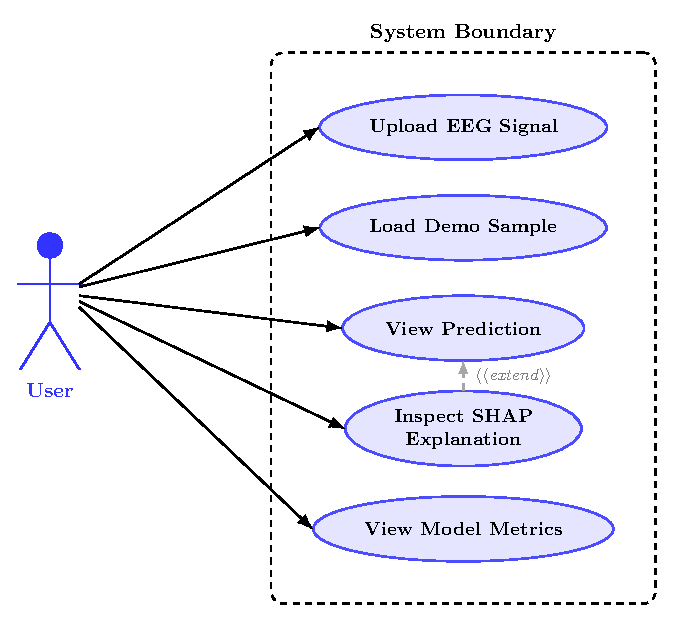
\includegraphics[width=0.9\textwidth]{images/use_case.pdf}
\caption{Use Case Diagram: EpiDetect System.}
\label{fig:usecase}
\end{figure}

\textbf{Actors:}
\begin{enumerate}
    \item \textbf{User:} Initiates EEG analysis through the web interface.
\end{enumerate}

\textbf{Process:} The user either uploads a CSV/TXT file containing raw EEG values or loads a demo sample from the Bonn dataset. The system preprocesses the signal, extracts features, runs the ensemble classifier, and displays the prediction along with a confidence score. The user can then navigate to the explanation section to view the SHAP summary plot and feature importance charts, or view global model performance metrics.

\subsection{Requirement Prioritisation}

\begin{enumerate}
    \item \textbf{Must Have:} Signal upload, preprocessing, feature extraction, classification, prediction display.
    \item \textbf{Should Have:} SHAP-based per-input explanation, global feature importance, model metrics dashboard.
    \item \textbf{Could Have:} Multi-file batch prediction, exportable reports.
    \item \textbf{Won't Have (this version):} Real-time streaming EEG support, multi-channel electrode handling.
\end{enumerate}

\section{Software Requirement Specification (SRS)}

\subsection{Purpose}
This SRS defines the functional and non-functional requirements that the EpiDetect system must satisfy, serving as a reference for development, testing, and evaluation.

\subsection{Functional Requirements}

Table~\ref{tab:funcreq} lists the eleven functional requirements of the EpiDetect system, each specifying a capability the system must provide to fulfil its intended purpose.

\begin{table}[htbp]
\centering
\caption{Functional Requirements.}
\label{tab:funcreq}
\begin{tabular}{|c|p{4cm}|p{6.5cm}|}
\hline
\textbf{ID} & \textbf{Requirement} & \textbf{Description} \\
\hline
FR1 & EEG Signal Input & The system must accept EEG data via file upload (CSV/TXT) or demo sample loading. \\
\hline
FR2 & Signal Preprocessing & The system must apply bandpass filtering and z-score normalization to the input signal. \\
\hline
FR3 & Feature Extraction & The system must extract 720 features across wavelet, time, frequency, and nonlinear domains. \\
\hline
FR4 & Feature Scaling & The system must apply StandardScaler normalization before classification. \\
\hline
FR5 & Feature Selection & The system must apply the saved feature selection mask to reduce dimensionality. \\
\hline
FR6 & Classification & The ensemble model must produce a seizure probability and a binary prediction (seizure/normal). \\
\hline
FR7 & Confidence Display & The prediction confidence must be shown as a percentage alongside the result. \\
\hline
FR8 & SHAP Explainability & The system must generate SHAP-based feature importance plots and summary visualizations for model transparency. \\
\hline
FR9 & Global SHAP \& Importance & The system must serve precomputed SHAP summary and feature importance plots. \\
\hline
FR10 & Metrics Endpoint & The system must expose saved cross-validation metrics via a REST endpoint. \\
\hline
FR11 & Health Check & The API must provide a health endpoint indicating model readiness. \\
\hline
\end{tabular}
\end{table}

\subsection{Non-Functional Requirements}

Table~\ref{tab:nonfuncreq} defines the non-functional requirements that govern the quality attributes of the system, including performance, reliability, maintainability, and extensibility.

\begin{table}[htbp]
\centering
\caption{Non-Functional Requirements.}
\label{tab:nonfuncreq}
\begin{tabular}{|c|p{4cm}|p{6.4cm}|}
\hline
\textbf{ID} & \textbf{Requirement} & \textbf{Description} \\
\hline
NFR1 & Performance & Single-signal prediction should complete within 5 seconds, including SHAP computation. \\
\hline
NFR2 & Reliability & The system should handle malformed inputs gracefully with informative error messages. \\
\hline
NFR3 & Usability & The web interface should be intuitive enough for users with no programming background. \\
\hline
NFR4 & Maintainability & Modular codebase with each pipeline stage in its own directory for easy updates. \\
\hline
NFR5 & Portability & The backend must run on any system with Python 3.8+ installed. \\
\hline
NFR6 & Reproducibility & Fixed random seeds and deterministic splits must ensure identical results across runs. \\
\hline
NFR7 & Extensibility & New classifiers or feature types must be addable without modifying existing modules. \\
\hline
\end{tabular}
\end{table}

\section{Hardware, Software Requirements, and Version Control}

The entire project is managed using Git for version tracking, with the repository hosted on GitHub. Each significant change is committed with a descriptive message, and the codebase is organized into clearly separated directories for backend modules, frontend assets, and documentation. Table~\ref{tab:hwsw} lists the hardware and software requirements needed to develop and run the EpiDetect system. The table is significant because every entry is a deliberately conservative requirement: the system targets a typical student or clinician laptop, with no GPU, no cloud account, and no commercial licences, which is what makes the deployment feasibility argument in Section 3.1 hold.

\begin{table}[htbp]
\centering
\renewcommand{\arraystretch}{1.3}
\caption{Hardware and Software Specifications.}
\label{tab:hwsw}
\begin{tabular}{|p{4cm}|p{7.5cm}|}
\hline
\textbf{Category} & \textbf{Specification} \\
\hline
Operating System & Windows 10/11, macOS, or Linux \\
\hline
Python Version & 3.8 or higher \\
\hline
RAM & 8~GB minimum (16~GB recommended) \\
\hline
Storage & 500~MB for code, model artifacts, and dataset \\
\hline
Key Libraries & scikit-learn, NumPy, SciPy, SHAP, Flask, Matplotlib, Joblib \\
\hline
Frontend & Any modern web browser (Chrome, Firefox, Edge) \\
\hline
\end{tabular}
\end{table}

        \chapter{System Design}
        
This chapter describes the overall architecture and design of the EpiDetect system. The discussion covers the end-to-end processing pipeline, the data flow through the system, and the design of each individual module. Each diagram is intentionally placed alongside the descriptive text that introduces it, so the reader does not have to flip pages to follow the design.

\section{System Architecture Overview}

The EpiDetect system follows a modular, layered architecture where each processing stage is encapsulated in its own module. Data flows sequentially from raw EEG input through preprocessing, feature extraction, classification, and explanation. The overall architecture is presented in Figure~\ref{fig:sysarch}.

The architecture in Figure~\ref{fig:sysarch} is significant because it makes the boundary between the offline training pipeline (top vertical chain) and the online inference path (the Flask REST API and Web Dashboard at the bottom) explicit. The trained ensemble in the centre is the single artifact shared between the two paths, which is why the SHAP explainer attaches to it directly rather than to the raw signal.

\begin{figure}[ht]
\centering
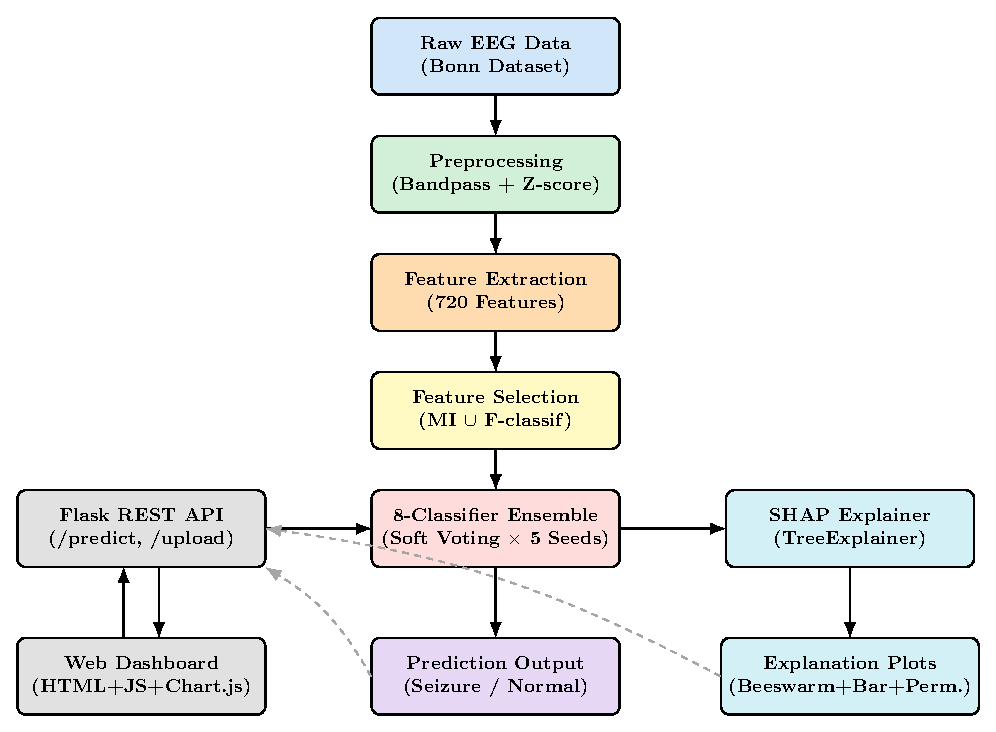
\includegraphics[width=0.78\textwidth]{images/sys_architecture.pdf}
\caption{System Architecture of the EpiDetect Pipeline.}
\label{fig:sysarch}
\end{figure}

\section{Process Flow of the Pipeline}

Figure~\ref{fig:processflow} illustrates the end-to-end process flow from the moment a user submits an EEG signal to the point where a prediction and explanation are displayed. Unlike the architectural view in Figure~\ref{fig:sysarch}, which captures the static layering of components, the process flow emphasises the temporal order in which each stage runs at inference time. This is important because each stage strictly depends on the output of the previous one; a missing or malformed intermediate output halts the pipeline.

\begin{figure}[H]
\centering
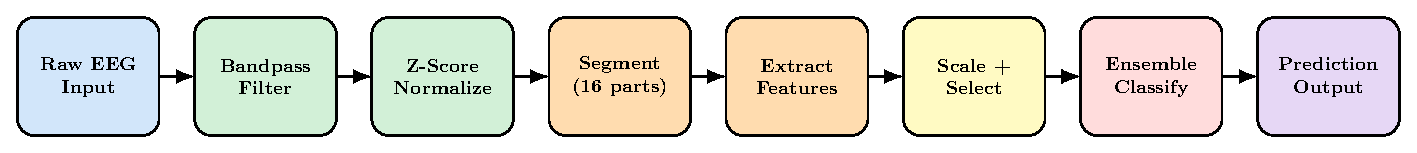
\includegraphics[width=\textwidth]{images/process_flow.pdf}
\caption{Process Flow Diagram: end-to-end signal processing pipeline.}
\label{fig:processflow}
\end{figure}

\section{Data Flow Diagram}

Figure~\ref{fig:dfd} presents a Level-1 data flow diagram showing how data moves between the major components of the system. The diagram makes two design properties visible at a glance. First, the trained model store (D2) feeds only the classification process and not the feature extractor, which is exactly the runtime relationship: features are computed from the input signal, while weights are loaded into the classifier. Second, the explanation process (4.0) closes the loop by routing both the prediction and its SHAP-based justification back to the user, which is the project's contribution toward clinical transparency.

\begin{figure}[H]
\centering
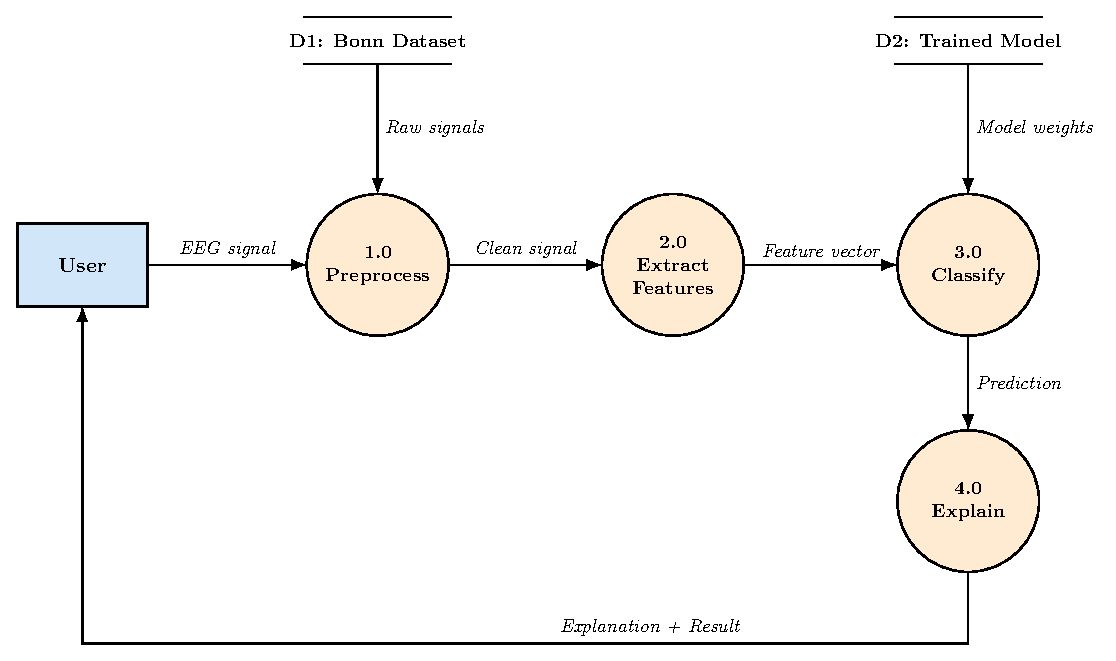
\includegraphics[width=0.95\textwidth]{images/dfd.pdf}
\caption{Level-1 Data Flow Diagram (Yourdon notation).}
\label{fig:dfd}
\end{figure}

\section{Activity Diagram}

Figure~\ref{fig:activity} presents the activity diagram for the EpiDetect prediction workflow, showing the sequence of operations along with the two key decision points that govern the processing path. The first decision (\textit{Valid Signal?}) acts as an input guard, returning an error before any processing if the uploaded file is malformed; this protects the downstream stages from spurious computation. The second decision (\textit{Prob $\geq 0.5$?}) converts the ensemble's continuous probability output into the binary clinical label that the dashboard displays. Note that the activity diagram intentionally treats the eight-classifier ensemble and the five-seed averaging as a single atomic activity (\textit{Run Ensemble (5 Seeds)}), because at the workflow level the user does not distinguish between the constituent classifiers. The internal structure of that activity is documented separately in the ensemble classification module design (Section~4.7.5).

\begin{figure}[H]
\centering
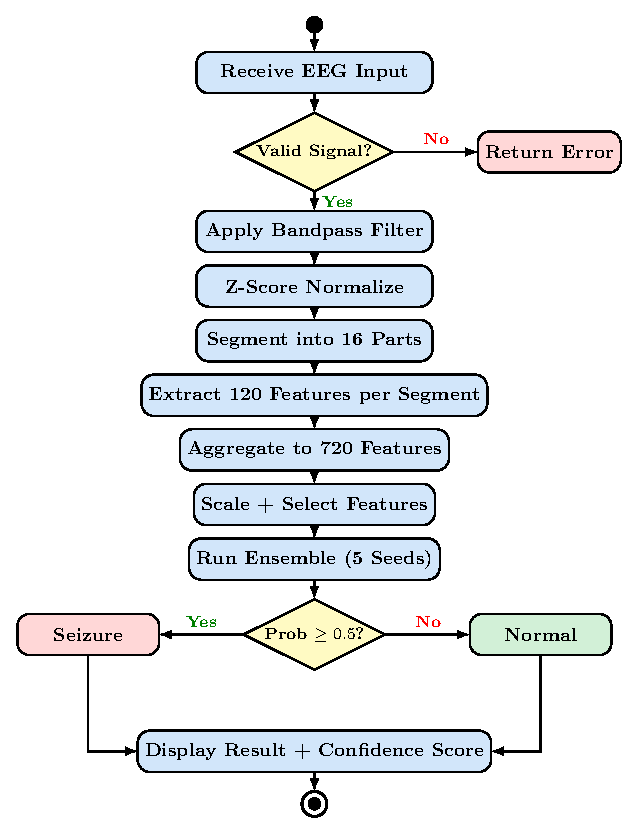
\includegraphics[width=0.55\textwidth]{images/activity_diagram.pdf}
\caption{Activity Diagram: EEG Prediction Workflow.}
\label{fig:activity}
\end{figure}

\section{Sequence Diagram}

Figure~\ref{fig:sequence} illustrates the interaction between the main components of the system during a typical prediction request. The user initiates a file upload through the browser, which communicates with the Flask API. The API delegates processing to the backend modules in sequence and returns the final result. The diagram is significant in two ways. First, it identifies the Flask API as the single orchestrator at inference time: every component except the User and Frontend communicates only through the API, which keeps the frontend stateless and the backend modules independently testable. Second, it makes the synchronous nature of the request-response cycle explicit: the API blocks on each backend stage in turn, so an error or delay in any one stage immediately surfaces in the JSON response delivered to the user. The dashed return arrows show that responses follow the inverse of the call chain, which means there is no out-of-band notification path; everything the user sees comes from the single response to the original POST request.

\begin{figure}[H]
\centering
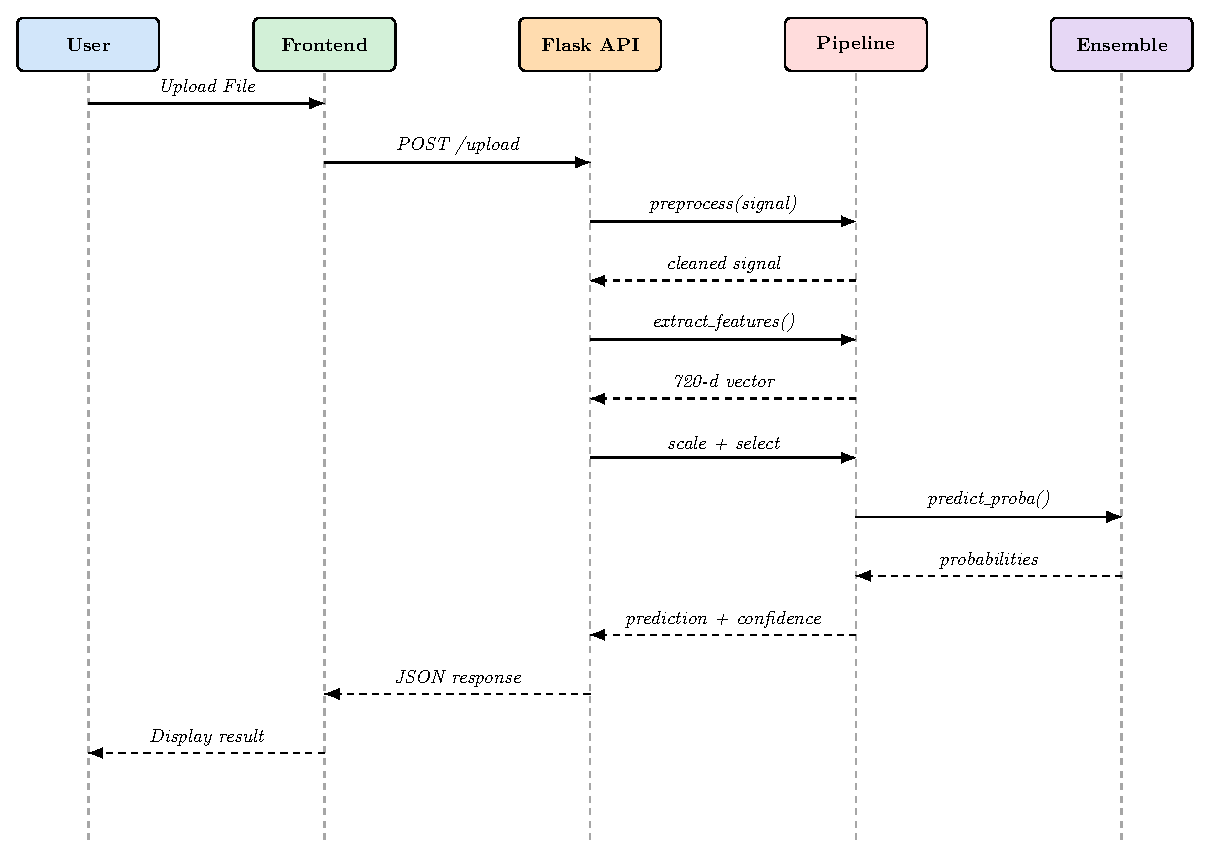
\includegraphics[width=\textwidth]{images/sequence_diagram.pdf}
\caption{Sequence Diagram: Signal Upload and Prediction.}
\label{fig:sequence}
\end{figure}

\section{Module Dependency Diagram}

Figure~\ref{fig:moduledep} shows the dependency relationships between the backend Python modules. The graph is deliberately a directed acyclic graph: \texttt{main.py} (the training entry point) depends only on the \texttt{cross\_validation} orchestrator, while \texttt{app.py} (the Flask inference entry point) depends on the four modules it directly invokes at runtime, namely \texttt{preprocess}, \texttt{extract}, \texttt{ensemble}, and \texttt{explainer}. The four worker modules and the \texttt{loader} all import constants from \texttt{settings} (paths, hyperparameters, feature counts), so each of them has an outgoing edge into \texttt{settings} at the bottom of the diagram. Every other module depends downward only, and \texttt{settings} has zero outgoing edges. This layered structure was chosen because it allows any individual module to be swapped (for example, replacing the ensemble with a different classifier) without recompiling or modifying any other module.

\begin{figure}[H]
\centering
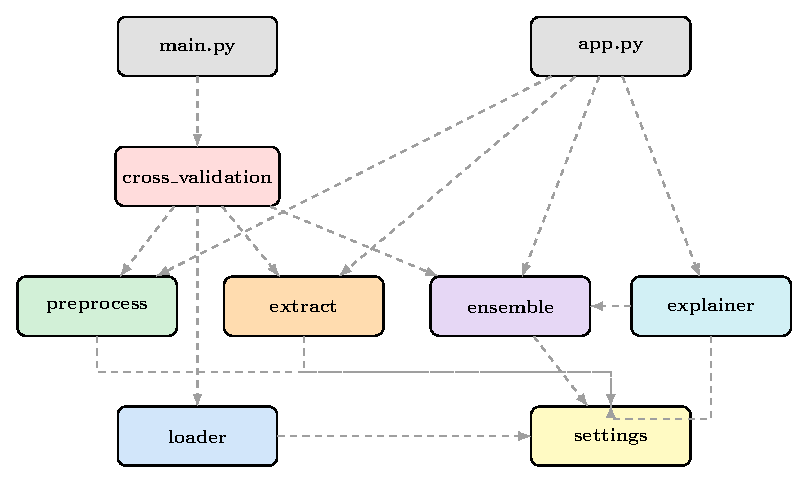
\includegraphics[width=0.85\textwidth]{images/module_dependency.pdf}
\caption{Module Dependency Diagram.}
\label{fig:moduledep}
\end{figure}

\section{Module Design}

This section describes the design of each module in the pipeline.

\subsection{Data Loading Module}

The data loader reads the Bonn University EEG dataset from disk. Each of the five clinical sets (Z, O, N, F, S) is stored as a collection of text files, where each file contains 4097 amplitude values sampled at 173.61~Hz. The loader scans the dataset directory, identifies each set by its starting letter, reads all files in that set, and assigns the appropriate binary label (0 for non-seizure, 1 for seizure).

\subsection{Preprocessing Module}

The preprocessing module applies two transformations to each raw signal. First, a fourth-order Butterworth bandpass filter with cutoff frequencies at 0.5~Hz and 85~Hz removes DC drift and high-frequency noise. The filter is applied using zero-phase filtering (\texttt{filtfilt}) so that no time delay is introduced. Second, z-score normalization is applied to standardize each signal to zero mean and unit variance. This ensures that the feature extraction pipeline receives signals on a consistent scale.

\subsection{Feature Extraction Module}

This module is the most computationally intensive part of the pipeline. Each signal (4097 samples) is split into 16 equal segments. For each segment, 120 features are computed across four domains:

\begin{enumerate}
    \item \textbf{DWT Features:} Five sub-bands (one approximation, four detail levels) each described by 15 statistics: mean, max, min, variance, wavelet entropy, energy, max absolute, min absolute, standard deviation, kurtosis, skewness, RMS, zero-crossing rate, mean absolute deviation, and coefficient of variation.

    \item \textbf{Time-Domain Features:} Mean, standard deviation, max, min, peak-to-peak range, kurtosis, skewness, RMS, zero-crossing rate, mean absolute value, Hjorth mobility, Hjorth complexity, line length, Teager energy, IQR, median absolute deviation, and variance.

    \item \textbf{Frequency-Domain Features:} Total power, peak frequency, mean frequency, median frequency, spectral entropy, absolute and relative band powers for delta through gamma, theta/alpha ratio, delta/beta ratio, slow/fast ratio, spectral edge frequencies at 85\% and 95\%, spectral centroid, and spectral spread.

    \item \textbf{Nonlinear Features:} Sample entropy, permutation entropy (orders 3 and 4), detrended fluctuation analysis (DFA), Higuchi fractal dimension, and a rescaled-range Hurst exponent estimate.
\end{enumerate}

After computing 120 features per segment across 16 segments, the values are aggregated using six statistics: mean, standard deviation, maximum, minimum, median, and interquartile range. This yields $120 \times 6 = 720$ features per signal.

Figure~\ref{fig:featurearch} shows the feature extraction architecture. The diagram is important for understanding the dimensionality bookkeeping: the 720 figure quoted throughout this report is not arbitrary, but the product of 120 per-segment features and 16 segments, summarised through 6 aggregation statistics. Any change to one of these three numbers propagates to the final feature count.

\begin{figure}[H]
\centering
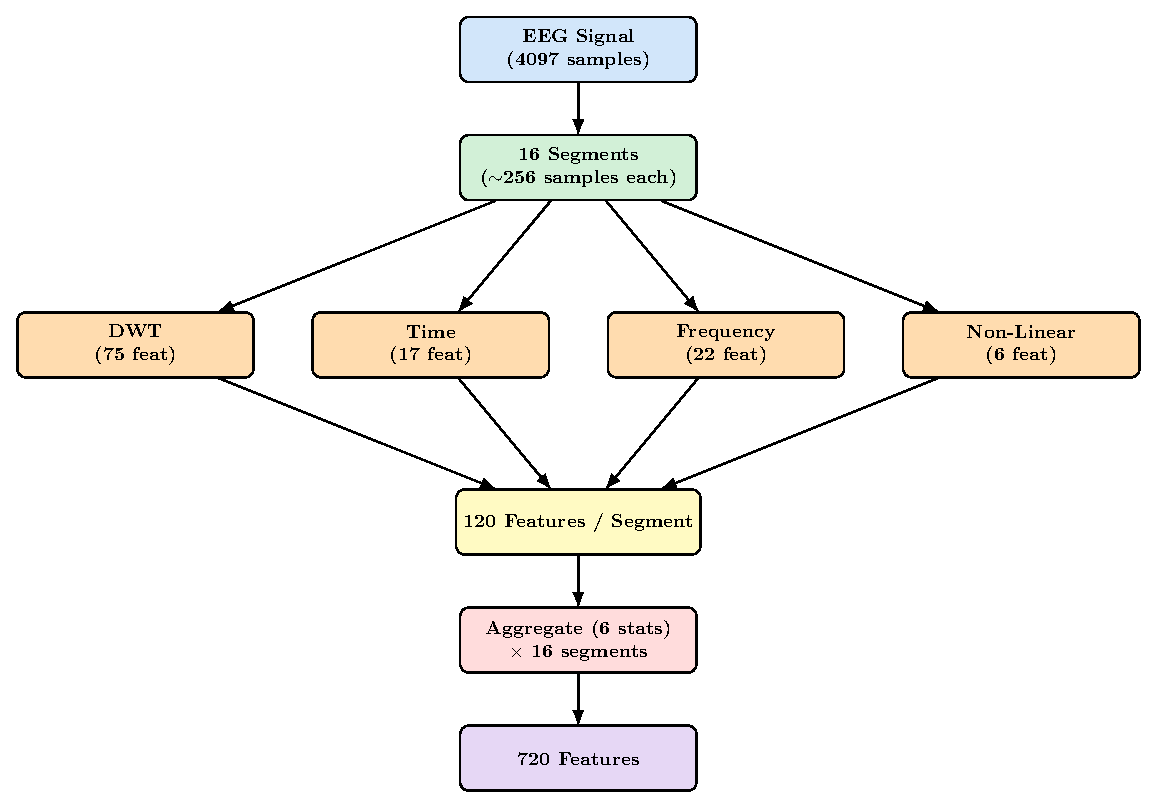
\includegraphics[width=0.7\textwidth]{images/feature_arch.pdf}
\caption{Feature Extraction Architecture.}
\label{fig:featurearch}
\end{figure}

\subsection{Feature Selection Module}

The feature selection module applies a union-based strategy. Two separate selectors, Mutual Information and ANOVA F-classif, each identify the top-$k$ (200) most informative features. The union of both sets is taken, yielding a feature subset that retains any feature considered important by \textit{either} method. This typically produces a subset of 280 to 330 features, which is considerably smaller than the original 720 but retains a broader view of relevance than a single selector alone.

\subsection{Ensemble Classification Module}

The classification module constructs a soft-voting ensemble of eight classifiers. Each classifier brings a different inductive bias, summarised in Table~\ref{tab:classifiers}. The table is important because it makes explicit \textit{why} eight different classifiers are combined rather than simply tuning a single one: each row identifies a distinct learning bias, and the soft-voting scheme ensures that no single bias dominates the final probability estimate.

\begin{table}[htbp]
\centering
\renewcommand{\arraystretch}{1.3}
\caption{Eight Classifiers in the Ensemble.}
\label{tab:classifiers}
\resizebox{\textwidth}{!}{%
\begin{tabular}{|c|p{5cm}|p{8.5cm}|}
\hline
\textbf{No.} & \textbf{Classifier} & \textbf{Role in the Ensemble} \\
\hline
1 & Random Forest (RF) & Bagging ensemble; robust, low variance. \\
\hline
2 & Extra Trees (ET) & More randomized than RF; further reduces overfitting. \\
\hline
3 & Hist. Gradient Boosting (HGB) & Fast boosting algorithm; handles large feature sets. \\
\hline
4 & Gradient Boosting (GBM) & Sequential boosting; corrects residual errors. \\
\hline
5 & AdaBoost & Focuses on hard to classify samples. \\
\hline
6 & SVM (RBF kernel) & Finds optimal decision boundaries in high-dimensional space. \\
\hline
7 & MLP (Neural Network) & Learns nonlinear feature combinations. \\
\hline
8 & K-Nearest Neighbours (KNN) & Captures local neighbourhood patterns. \\
\hline
\end{tabular}%
}
\end{table}

The ensemble uses \textit{soft voting}: each classifier outputs a probability for the seizure class, and the final probability is the average across all eight. To further reduce variance, the entire ensemble is trained five times with different random seeds, and the final prediction is the average of all five runs.

\subsection{XAI Module}

The explainability module uses SHAP (SHapley Additive exPlanations)~\citep{lundberg2017unified} to provide three types of explanations:

\begin{enumerate}
    \item \textbf{Global Feature Importance:} Averaged across all tree-based estimators in the ensemble, this shows which features the model relies on most heavily overall.

    \item \textbf{SHAP Summary and Bar Plots:} Multi-tree SHAP values are computed by averaging TreeExplainer outputs from the Random Forest, Extra Trees, and Gradient Boosting components. The summary beeswarm plot shows how each feature's value influences the prediction across all test samples, while the bar plot ranks features by mean absolute SHAP value.

    \item \textbf{Permutation Importance:} Each feature's values are randomly shuffled and the resulting drop in accuracy is measured using the full eight-classifier ensemble, revealing which features are genuinely critical to the model's performance.
\end{enumerate}

\subsection{REST API and Web Dashboard}

The Flask-based REST API serves as the bridge between the trained model and the user-facing dashboard. It exposes endpoints for health checking, signal prediction, file upload, and XAI plot retrieval. The frontend, built with vanilla HTML, CSS, and JavaScript (with Chart.js for data visualization), connects to these endpoints and presents predictions, confidence scores, and explanation plots in an interactive interface.

\section{Project Directory Structure}

Table~\ref{tab:dirstructure} shows the modular directory organization of the codebase. The structure mirrors the module dependency diagram in Figure~\ref{fig:moduledep}: each row corresponds to a node in the graph, and the directory hierarchy reflects the layered grouping (configuration at the top, workers in the middle, entry points at the bottom).

\begin{table}[htbp]
\centering
\renewcommand{\arraystretch}{1.15}
\caption{Project Directory Structure.}
\label{tab:dirstructure}
\resizebox{\textwidth}{!}{%
\begin{tabular}{|p{7cm}|p{7cm}|}
\hline
\textbf{Path} & \textbf{Purpose} \\
\hline
\texttt{backend/config/settings.py} & All constants and hyperparameters \\
\hline
\texttt{backend/data/loader.py} & Bonn dataset loader \\
\hline
\texttt{backend/preprocessing/preprocess.py} & Bandpass filter + z-score normalization \\
\hline
\texttt{backend/features/extract.py} & 720 feature extraction pipeline \\
\hline
\texttt{backend/models/ensemble.py} & 8 classifier soft-voting ensemble \\
\hline
\texttt{backend/training/cross\_validation.py} & 10-fold CV + model saving \\
\hline
\texttt{backend/xai/explainer.py} & SHAP-based explanations \\
\hline
\texttt{backend/main.py} & Full training pipeline entry point \\
\hline
\texttt{backend/app.py} & Flask REST API \\
\hline
\texttt{frontend/index.html} & Web dashboard \\
\hline
\texttt{frontend/js/app.js} & Frontend logic + Chart.js \\
\hline
\texttt{frontend/css/style.css} & Dashboard styling \\
\hline
\end{tabular}%
}
\end{table}

        \chapter{Implementation}
        
This chapter describes the implementation of each module in detail, including formal algorithms for the core processing steps. The system is implemented in Python 3.8+ on the backend and vanilla HTML/CSS/JavaScript on the frontend.

\section{Signal Preprocessing}

The preprocessing module operates on the raw 4097-sample signals loaded from the Bonn dataset. Two operations are applied sequentially.

\subsection{Bandpass Filtering}

A fourth-order Butterworth bandpass filter is designed with cutoff frequencies at 0.5~Hz and 85~Hz. The lower cutoff removes DC drift and slow baseline wander, while the upper cutoff attenuates high-frequency noise above the usable EEG range. The Nyquist frequency for the Bonn dataset is $173.61 / 2 = 86.8$~Hz.

Filtering is performed using SciPy's \texttt{filtfilt} function, which applies the filter both forward and backward. This zero-phase approach ensures that no time delay is introduced, which is important for preserving the temporal alignment of features across segments.

\subsection{Z-Score Normalization}

After filtering, each signal is normalized by subtracting its mean and dividing by its standard deviation. This brings all signals to a common scale (mean~=~0, std~=~1), ensuring that the feature extraction pipeline is not biased by differences in absolute amplitude across recordings.

\section{Multi-Domain Feature Extraction}

Feature extraction is the most computationally intensive module. Each signal is processed through four domain-specific extractors, and the resulting per-segment features are aggregated into a single vector.

\subsection{Signal Segmentation}

Each 4097-sample signal is divided into 16 non-overlapping segments of approximately 256 samples each. Computing features at the segment level captures local temporal variations that a whole-signal analysis would average out. For instance, a brief burst of high-frequency activity in one segment would contribute to that segment's spectral features even if the surrounding segments are calm.

\subsection{Discrete Wavelet Transform}

A manual implementation of the Daubechies-4 (DB4) wavelet is used, avoiding external wavelet library dependencies. The signal is decomposed into 4 levels, producing 5 sub-bands:

\begin{itemize}
    \item \textbf{A4} (Approximation): captures delta-range activity (0--5~Hz)
    \item \textbf{D4} (Detail Level 4): captures theta/alpha activity (5--11~Hz)
    \item \textbf{D3} (Detail Level 3): captures alpha/beta activity (11--22~Hz)
    \item \textbf{D2} (Detail Level 2): captures beta/gamma activity (22--43~Hz)
    \item \textbf{D1} (Detail Level 1): captures gamma activity (43--87~Hz)
\end{itemize}

For each sub-band, 15 statistical measures are computed: mean, maximum, minimum, variance, wavelet entropy, energy, max absolute value, min absolute value, standard deviation, kurtosis, skewness, RMS, zero-crossing rate, mean absolute deviation, and coefficient of variation. Together these statistics capture the amplitude distribution, energy concentration, and signal regularity within each frequency band, providing a rich multi-scale characterisation of seizure-related spectral activity.

\subsection{Time-Domain Features}

Seventeen time-domain features are computed for each segment, including Hjorth parameters (mobility, complexity)~\citep{hjorth1970eeg}, Teager energy operator~\citep{kaiser1990simple}, line length, and standard statistical measures. The Hjorth parameters, defined in Equations~\eqref{eq:hjorth_act}--\eqref{eq:hjorth_comp}, characterise the signal in terms of power, frequency content, and waveform complexity:

\begin{align}
    \text{Activity} &= \text{Var}(x) \label{eq:hjorth_act} \\[0.5em]
    \text{Mobility} &= \sqrt{\frac{\text{Var}(x')}{\text{Var}(x)}} \label{eq:hjorth_mob} \\[0.5em]
    \text{Complexity} &= \frac{\text{Mobility}(x')}{\text{Mobility}(x)} \label{eq:hjorth_comp}
\end{align}

where $x'$ denotes the first derivative of the signal segment. Activity represents signal power, Mobility reflects mean frequency, and Complexity quantifies how close the signal shape is to a pure sine wave.

The Teager energy operator, defined in Equation~\eqref{eq:teager}, responds to rapid changes in both amplitude and frequency and is therefore sensitive to the high-energy bursts characteristic of ictal activity:

\medskip
\begin{equation}
    \Psi[x(n)] = x(n)^2 - x(n-1) \cdot x(n+1)
    \label{eq:teager}
\end{equation}
\medskip

\subsection{Frequency-Domain Features}

The FFT-derived features include total spectral power, peak frequency, mean frequency, median frequency, spectral entropy, and absolute and relative band powers for the five standard EEG bands (delta, theta, alpha, beta, gamma). Additionally, band power ratios (theta/alpha, delta/beta, slow/fast) and spectral edge frequencies at the 85th and 95th percentiles are computed. This gives 22 frequency-domain features per segment.

\subsection{Nonlinear Features}

Six nonlinear complexity measures are extracted:
\begin{enumerate}
    \item \textbf{Sample Entropy}~\citep{richman2000physiological}: quantifies signal unpredictability through template matching. It is defined as:
    \begin{equation}
        \text{SampEn}(m, r, N) = -\ln\frac{A}{B}
        \label{eq:sampen}
    \end{equation}
    where $A$ is the number of template vector pairs of length $m+1$ within tolerance $r$, $B$ is the count for length $m$, and $N$ is the signal length. Lower values indicate more regular, predictable signals; seizure EEG typically exhibits elevated entropy.

    \item \textbf{Permutation Entropy (orders 3 and 4)}~\citep{bandt2002permutation}: quantifies complexity through ordinal pattern analysis. It is defined as:
    \begin{equation}
        H_{\text{PE}} = -\sum_{\pi} p(\pi) \ln p(\pi)
        \label{eq:perment}
    \end{equation}
    where the sum runs over all ordinal patterns $\pi$ of a given order $m$, and $p(\pi)$ is the relative frequency of each pattern. Computing at orders 3 and 4 captures complexity at different temporal scales.

    \item \textbf{Detrended Fluctuation Analysis (DFA)}~\citep{peng1994mosaic}: measures long-range temporal correlations by estimating the scaling exponent $\alpha$ from the relationship $F(n) \sim n^{\alpha}$, where $F(n)$ is the root-mean-square fluctuation over window size $n$ after local trend removal.

    \item \textbf{Higuchi Fractal Dimension}~\citep{higuchi1988approach}: measures signal roughness via the Higuchi algorithm with $k_{\max} = 8$. A higher fractal dimension indicates greater irregularity, which is a hallmark of ictal EEG.

    \item \textbf{Rescaled-Range (Hurst-like exponent)}: estimates long-range dependence using the cumulative sum approach. Values near 0.5 indicate a random process; deviations signal persistent or anti-persistent dynamics.
\end{enumerate}

\subsection{Segment Aggregation}

After computing 120 features per segment across 16 segments, the segment-level values are aggregated using six statistics: mean, standard deviation, maximum, minimum, median, and interquartile range. The final feature vector has $120 \times 6 = 720$ dimensions.

Algorithm~\ref{alg:feature} presents the complete feature extraction procedure.

\begin{algorithm}[ht]
\caption{Multi-Domain Feature Extraction}
\label{alg:feature}
\SetAlgoLined
\KwIn{EEG signal $\mathbf{x}$ of length 4097}
\KwOut{Feature vector $\mathbf{f}$ of length 720}
\BlankLine
$N_{\text{seg}} \leftarrow 16$\;
$L \leftarrow \lfloor |\mathbf{x}| / N_{\text{seg}} \rfloor$\;
$\mathbf{F}_{\text{seg}} \leftarrow$ empty matrix of size $N_{\text{seg}} \times 120$\;
\BlankLine
\For{$i \leftarrow 0$ \KwTo $N_{\text{seg}} - 1$}{
    $\mathbf{s} \leftarrow \mathbf{x}[iL : (i+1)L]$ \tcp*{Extract segment}
    \BlankLine
    $\mathbf{c} \leftarrow$ DWT-DB4 decompose $\mathbf{s}$ to depth 4\;
    $\mathbf{f}_{\text{dwt}} \leftarrow$ Compute 15 statistics for each of 5 sub-bands in $\mathbf{c}$\;
    \BlankLine
    $\mathbf{f}_{\text{time}} \leftarrow$ Compute time-domain statistics for $\mathbf{s}$\;
    $\mathbf{f}_{\text{freq}} \leftarrow$ Compute FFT-based spectral features for $\mathbf{s}$\;
    $\mathbf{f}_{\text{nl}} \leftarrow$ Compute nonlinear complexity features for $\mathbf{s}$\;
    \BlankLine
    $\mathbf{F}_{\text{seg}}[i] \leftarrow [\mathbf{f}_{\text{dwt}} \| \mathbf{f}_{\text{time}} \| \mathbf{f}_{\text{freq}} \| \mathbf{f}_{\text{nl}}]$\;
}
\BlankLine
\tcp{Aggregate across 16 segments}
$\mathbf{f} \leftarrow [\text{mean}(\mathbf{F}_{\text{seg}}) \| \text{std}(\mathbf{F}_{\text{seg}}) \| \max(\mathbf{F}_{\text{seg}}) \| \min(\mathbf{F}_{\text{seg}}) \| \text{median}(\mathbf{F}_{\text{seg}}) \| \text{IQR}(\mathbf{F}_{\text{seg}})]$\;
\BlankLine
\Return $\mathbf{f}$\;
\end{algorithm}

\section{Feature Selection}

Feature selection is handled through a union strategy. Two independent selectors are applied to the training data:

\begin{enumerate}
    \item \textbf{Mutual Information (MI):} Measures the mutual dependence between each feature and the target label. It captures both linear and nonlinear relationships.
    
    \item \textbf{ANOVA F-classif:} Computes the F-statistic for each feature, testing whether the feature distributions differ significantly between the seizure and non-seizure classes.
\end{enumerate}

Each selector identifies the top-200 features. The union of both sets creates a combined feature subset that retains any feature considered important by \textit{either} method. This typically results in 280--330 features, providing a broader perspective than a single selector while still substantially reducing dimensionality.

\section{Ensemble Classification and Multi-Seed Training}

The ensemble uses scikit-learn's~\citep{pedregosa2011scikit} \texttt{VotingClassifier} with \texttt{voting=`soft'}. Each of the eight classifiers outputs a probability for the seizure class, and the final probability is the unweighted average. The Random Forest and Extra Trees components follow Breiman's bagging formulation~\citep{breiman2001random}. Class imbalance (seizure signals constitute only 20\% of the dataset) is handled by assigning a weight of 4.0 to the minority class in classifiers that support class weights (RF, ET, HGB, SVM).

To reduce the variance caused by random initialization (which affects MLP, random forests, and boosting algorithms), the ensemble is trained five times with seeds $\{42, 123, 456, 789, 2024\}$. The five sets of probability outputs are averaged to produce the final prediction. A sample is classified as seizure if its averaged probability exceeds 0.5.

Algorithm~\ref{alg:ensemble} formalizes this multi-seed ensemble prediction procedure.

\begin{algorithm}[ht]
\caption{Multi-Seed Ensemble Prediction}
\label{alg:ensemble}
\SetAlgoLined
\KwIn{Training data $(\mathbf{X}_{\text{train}}, \mathbf{y}_{\text{train}})$, test data $\mathbf{X}_{\text{test}}$}
\KwOut{Predicted probabilities $\mathbf{p}$ for seizure class}
\BlankLine
$\mathcal{S} \leftarrow \{42, 123, 456, 789, 2024\}$  \tcp*{Seed set}
$\mathbf{P} \leftarrow$ empty list of probability vectors\;
\BlankLine
\ForEach{$s \in \mathcal{S}$}{
    $\mathcal{E}_s \leftarrow$ BuildEnsemble$(s)$ \tcp*{8 classifiers with seed $s$}
    
    \tcp{The ensemble contains: RF, ET, HGB, GBM, AdaBoost, SVM, MLP, KNN}
    
    Fit $\mathcal{E}_s$ on $(\mathbf{X}_{\text{train}}, \mathbf{y}_{\text{train}})$\;
    $\mathbf{p}_s \leftarrow \mathcal{E}_s.\text{predict\_proba}(\mathbf{X}_{\text{test}})[:, 1]$ \tcp*{Seizure prob.}
    Append $\mathbf{p}_s$ to $\mathbf{P}$\;
}
\BlankLine
$\mathbf{p} \leftarrow \text{mean}(\mathbf{P})$ \tcp*{Average across all seeds}
\BlankLine
\For{$j \leftarrow 0$ \KwTo $|\mathbf{p}| - 1$}{
    \eIf{$\mathbf{p}[j] \geq 0.5$}{
        $\hat{y}[j] \leftarrow$ Seizure\;
    }{
        $\hat{y}[j] \leftarrow$ Normal\;
    }
}
\BlankLine
\Return $\mathbf{p}$, $\hat{\mathbf{y}}$\;
\end{algorithm}

\section{Cross-Validation}

The model is evaluated using 10-fold stratified cross-validation. In each fold:

\begin{enumerate}
    \item \textbf{Scaling:} \texttt{StandardScaler} is fit on the training split and applied to both training and test splits.
    \item \textbf{Feature Selection:} The MI and F-classif selectors are fit on the training split. The union of their top-200 features is applied to both splits.
    \item \textbf{Training:} The multi-seed ensemble is trained on the selected features of the training split.
    \item \textbf{Evaluation:} Predictions on the test split are scored with accuracy, precision, recall, F1-score, AUC-ROC, specificity, and Cohen's kappa.
\end{enumerate}

Stratification ensures that each fold maintains approximately the same seizure-to-normal ratio as the full dataset (1:4). The scaler, feature indices, and trained ensemble from the final fold are saved to disk for use by the Flask API at inference time.

\section{SHAP-Based Explainability}

Two types of SHAP explanations are computed:

\subsection{Global Feature Importance}

The built-in \texttt{feature\_importances\_} attribute is extracted from each tree-based model in the ensemble (RF, ET, HGB, GBM, AdaBoost). Each model's importances are normalized to sum to 1, and then averaged across all five tree-based models. The top 20 features are plotted as a horizontal bar chart.

\subsection{Multi-Tree SHAP Analysis}

SHAP values are computed using \texttt{TreeExplainer} on the Random Forest, Extra Trees, and Gradient Boosting components of the ensemble. The SHAP values from these three models are averaged to produce a combined attribution that reflects the consensus of multiple tree-based learners. A summary beeswarm plot and a bar plot of mean absolute SHAP values are generated and saved for the top 20 features.

\subsection{Permutation Importance}

Permutation importance is computed using the full eight-classifier ensemble. For each feature, its values are randomly shuffled across the test set, and the resulting drop in accuracy is measured. Features whose shuffling causes a large accuracy drop are deemed important. This approach complements SHAP by covering all eight classifiers, including SVM, MLP, and KNN which are not covered by TreeExplainer.

\section{REST API Implementation}

The Flask API exposes the following endpoints:

\begin{table}[H]
\centering
\renewcommand{\arraystretch}{1.3}
\caption{REST API Endpoints.}
\label{tab:apiendpoints}
\resizebox{\textwidth}{!}{%
\begin{tabular}{|p{3.5cm}|p{1.5cm}|p{9cm}|}
\hline
\textbf{Endpoint} & \textbf{Method} & \textbf{Description} \\
\hline
\texttt{/health} & GET & Returns model readiness status. \\
\hline
\texttt{/demo} & GET & Loads a real EEG sample from the Bonn dataset; accepts query parameters for class selection. \\
\hline
\texttt{/predict} & POST & Accepts a JSON body with an \texttt{eeg} array; returns prediction, probability, and confidence score. \\
\hline
\texttt{/upload} & POST & Accepts a CSV or TXT file upload; returns the same prediction payload. \\
\hline
\texttt{/metrics} & GET & Returns saved cross-validation metrics as JSON. \\
\hline
\texttt{/xai/importance} & GET & Returns the feature importance bar chart as a PNG image. \\
\hline
\texttt{/xai/shap} & GET & Returns the SHAP summary beeswarm plot as a PNG image. \\
\hline
\texttt{/xai/shap-bar} & GET & Returns the SHAP bar plot as a PNG image. \\
\hline
\texttt{/xai/permutation} & GET & Returns the permutation importance plot as a PNG image. \\
\hline
\end{tabular}%
}
\end{table}

Cross-Origin Resource Sharing (CORS) is enabled globally so that the frontend, which may be served from a different origin, can communicate with the API without restrictions.

\section{Web Dashboard Implementation}

The frontend is a single-page application built with vanilla HTML, CSS, and JavaScript. Chart.js is used for the EEG signal waveform and bar charts. The interface is organized into four sections:

\begin{enumerate}
    \item \textbf{Analyze:} EEG signal input (upload or demo sample), waveform visualization, and prediction result with confidence ring.
    \item \textbf{Explain:} SHAP summary beeswarm, SHAP bar chart, feature importance, and permutation importance plots.
    \item \textbf{Performance:} Model metrics (accuracy, precision, recall, F1, AUC-ROC) displayed both as cards and bar charts.
    \item \textbf{About:} Project description, dataset details, ensemble architecture overview, and feature breakdown.
\end{enumerate}

        \chapter{Results and Analysis}
        
This chapter presents the experimental results obtained from the EpiDetect pipeline. All experiments were conducted on the Bonn University EEG dataset using 10-fold stratified cross-validation with multi-seed ensemble training.

\section{Experimental Setup}

\subsection{Dataset}

The Bonn University EEG dataset~\citep{andrzejak2001indications} consists of 500 single-channel EEG recordings, each containing 4097 amplitude values sampled at 173.61~Hz (approximately 23.6 seconds per recording). The data is organized into five clinical sets:

\begin{table}[htbp]
\centering
\renewcommand{\arraystretch}{1.3}
\caption{Bonn University EEG Dataset Composition.}
\label{tab:dataset}
\begin{tabular}{|c|c|l|c|c|}
\hline
\textbf{Set} & \textbf{Letter} & \textbf{Subject / State} & \textbf{Signals} & \textbf{Label} \\
\hline
A & Z & Healthy volunteer, eyes open & 100 & 0 (Normal) \\
\hline
B & O & Healthy volunteer, eyes closed & 100 & 0 (Normal) \\
\hline
C & N & Epileptic patient, seizure-free zone & 100 & 0 (Normal) \\
\hline
D & F & Epileptic patient, epileptogenic zone & 100 & 0 (Normal) \\
\hline
E & S & Epileptic patient, during seizure & 100 & 1 (Seizure) \\
\hline
\multicolumn{3}{|r|}{\textbf{Total}} & \textbf{500} & \\
\hline
\end{tabular}
\end{table}

The binary classification task groups Sets A--D as the non-seizure class (400 signals) and Set E as the seizure class (100 signals), producing a 4:1 class imbalance. This imbalance is addressed through class weighting (seizure weight = 4.0) in classifiers that support it.

Figure~\ref{fig:eegsignals} shows a representative EEG signal from each of the five sets. The healthy signals (Sets Z and O) exhibit relatively regular, low-amplitude oscillations. The inter-ictal recordings (Sets N and F), captured from epileptic patients between seizures, show slightly elevated irregularity. Set S (seizure) displays the characteristic high-amplitude, chaotic spikes that distinguish ictal activity from all other brain states.

\begin{figure}[htbp]
\centering
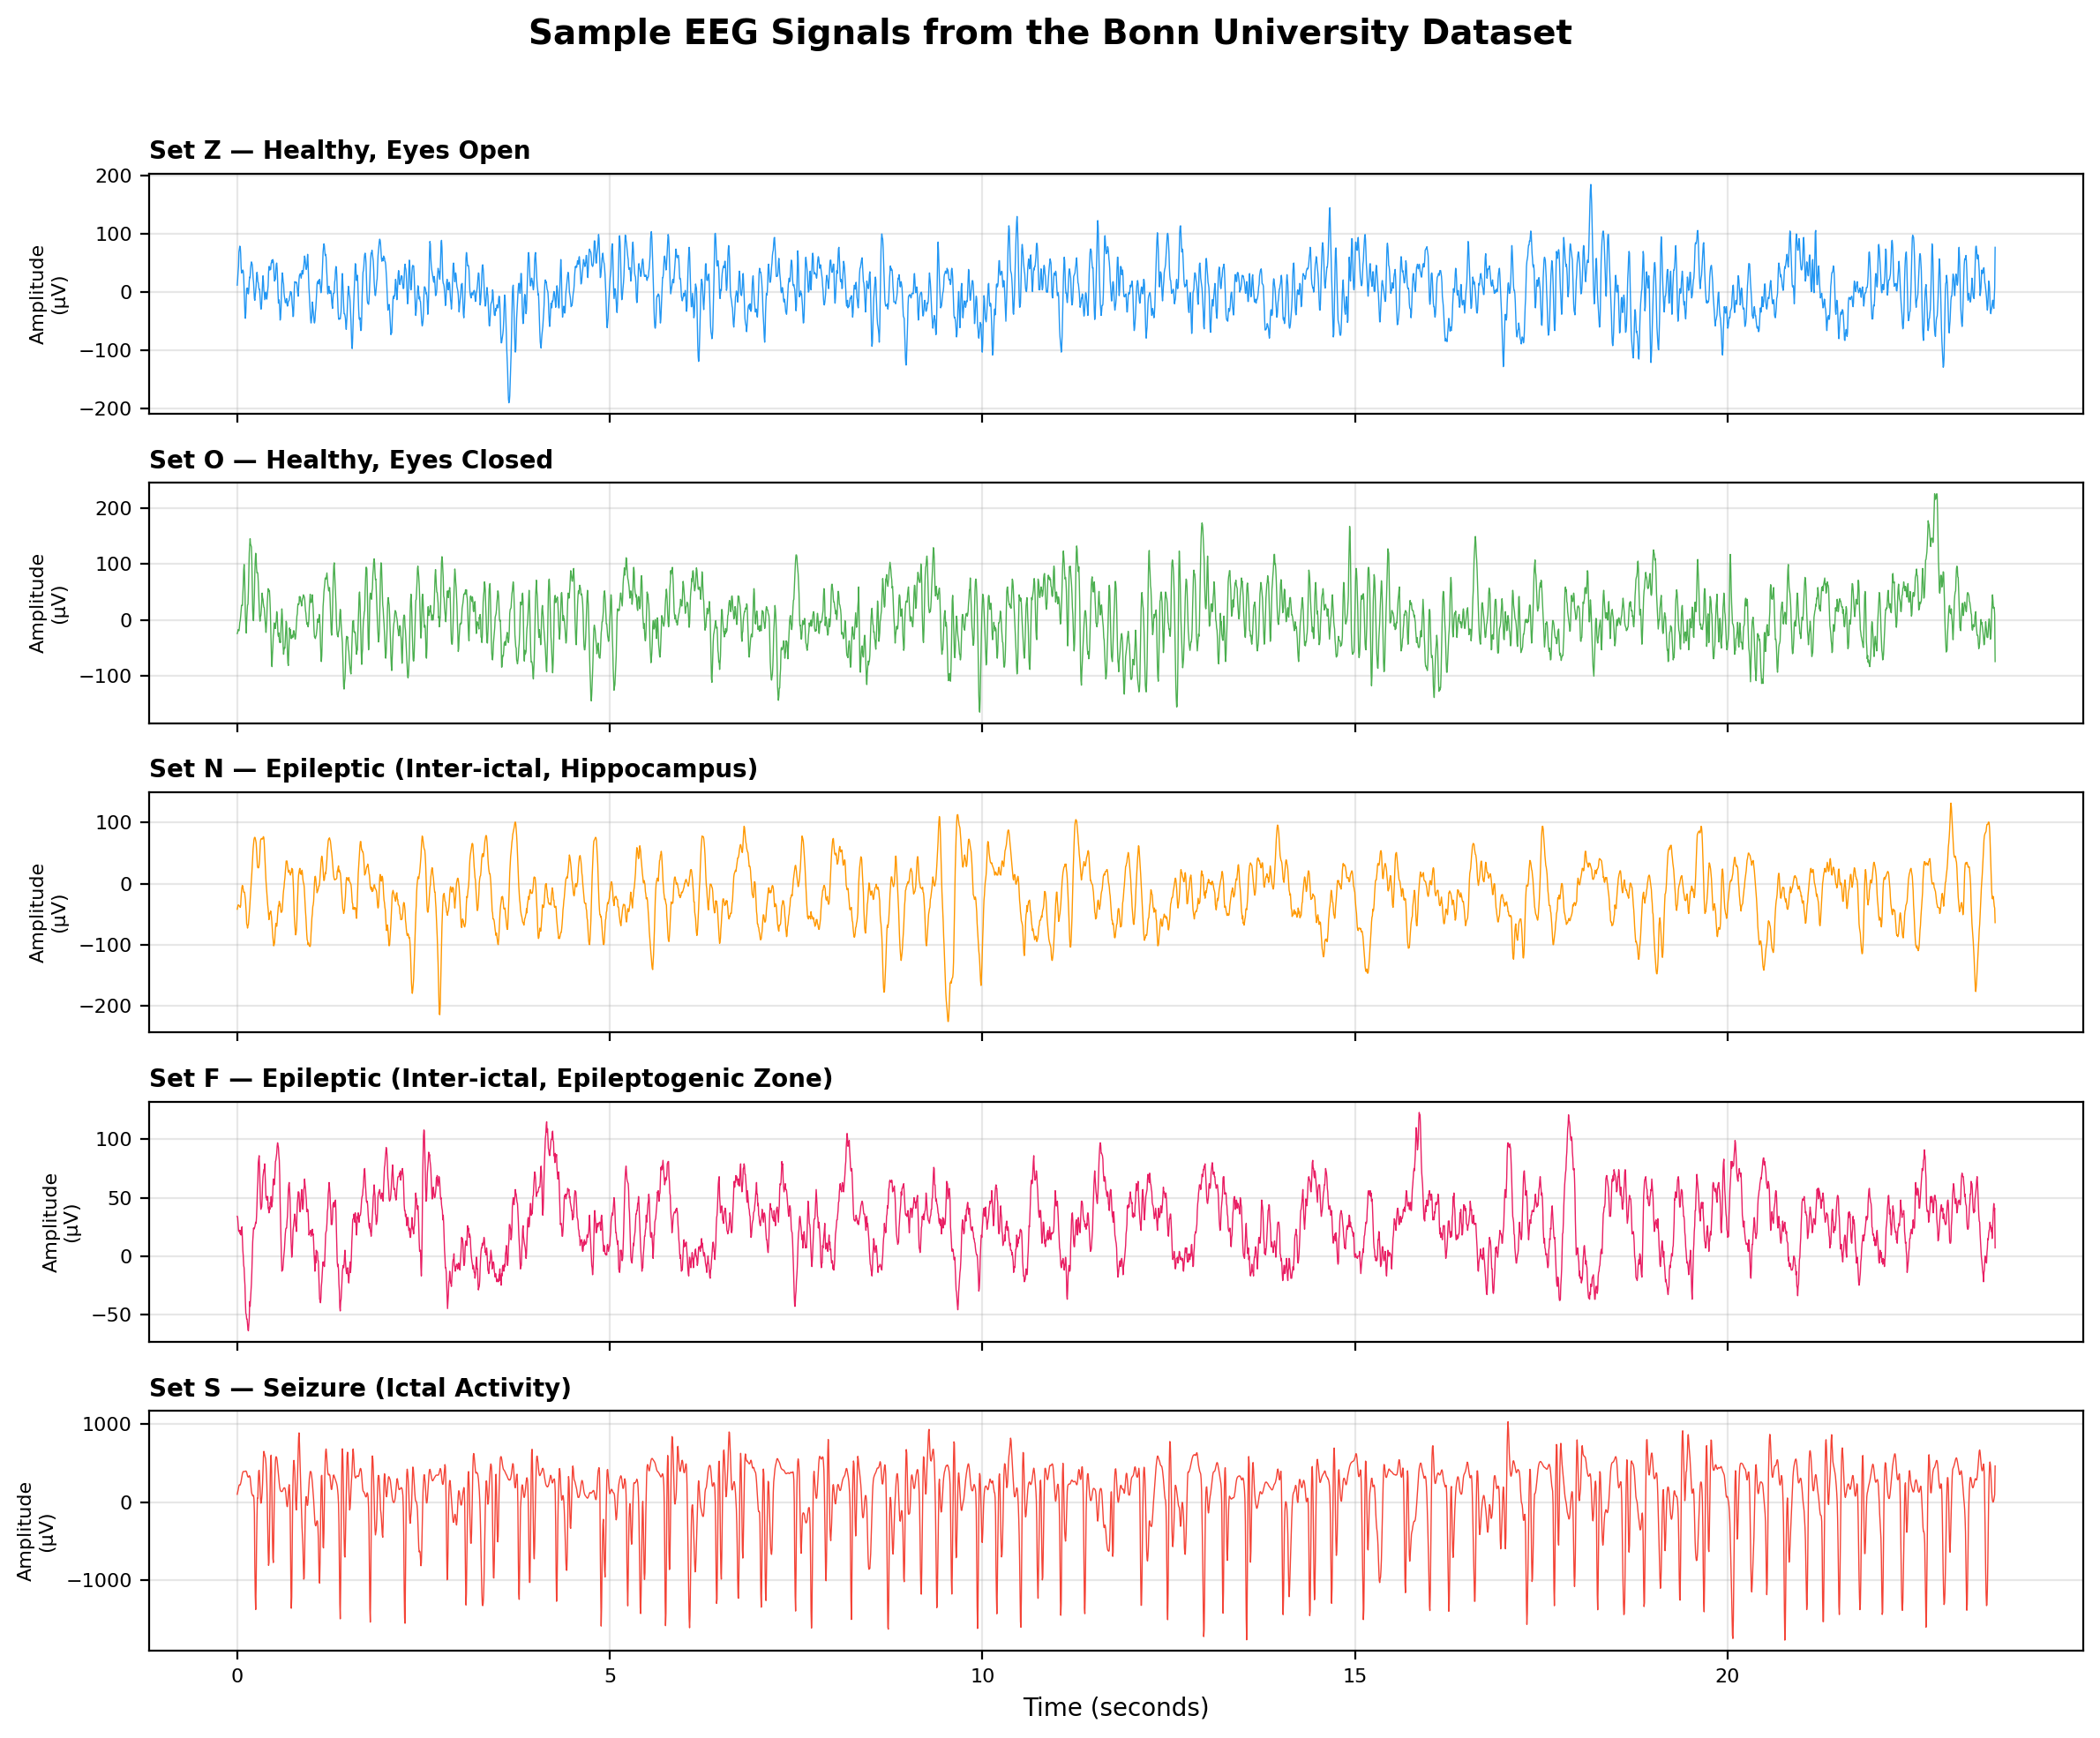
\includegraphics[width=\textwidth]{images/eeg_signals.png}
\caption{Sample EEG waveforms from each set of the Bonn University dataset.}
\label{fig:eegsignals}
\end{figure}

\subsection{Evaluation Protocol}

All results are reported under 10-fold stratified cross-validation. Stratification ensures that each fold preserves the 4:1 class ratio. Within each fold, the training data is used to fit the scaler, feature selectors, and classifiers, while the test data remains unseen until evaluation. Seven metrics are computed per fold: accuracy, precision, recall, F1-score, AUC-ROC, specificity, and Cohen's kappa.

\subsection{Training Configuration}

Key hyperparameters used in the experiments are listed below:

\begin{table}[htbp]
\centering
\renewcommand{\arraystretch}{1.25}
\caption{Training Hyperparameters.}
\label{tab:hyperparams}
\begin{tabular}{|l|l|}
\hline
\textbf{Parameter} & \textbf{Value} \\
\hline
Cross-validation folds & 10 (stratified) \\
\hline
Random seeds & \{42, 123, 456, 789, 2024\} \\
\hline
Feature selection (per method) & Top 200 \\
\hline
Classification threshold & 0.5 \\
\hline
Seizure class weight & 4.0 \\
\hline
RF / ET estimators & 500 trees \\
\hline
HGB iterations & 400 \\
\hline
GBM estimators & 300 \\
\hline
AdaBoost estimators & 200 \\
\hline
MLP architecture & (256, 128, 64) with early stopping \\
\hline
SVM kernel / C & RBF / 20.0 \\
\hline
KNN neighbours & 5 (distance weighted) \\
\hline
\end{tabular}
\end{table}

\section{Overall Classification Results}

Table~\ref{tab:overall} presents the mean and standard deviation of each metric across 10 folds.

\begin{table}[htbp]
\centering
\renewcommand{\arraystretch}{1.4}
\caption{Overall Classification Performance (10-Fold CV).}
\label{tab:overall}
\begin{tabular}{|l|c|}
\hline
\textbf{Metric} & \textbf{Mean $\pm$ Std (\%)} \\
\hline
Accuracy & 99.40 $\pm$ 0.92 \\
\hline
Precision & 99.09 $\pm$ 2.73 \\
\hline
Recall (Sensitivity) & 98.00 $\pm$ 4.00 \\
\hline
F1-Score & 98.47 $\pm$ 2.34 \\
\hline
AUC-ROC & 99.92 $\pm$ 0.23 \\
\hline
Specificity & 99.75 $\pm$ 0.75 \\
\hline
Cohen's Kappa & 98.10 $\pm$ 2.91 \\
\hline
\end{tabular}
\end{table}

The results show that the system achieves near-perfect classification on the Bonn dataset. The accuracy of 99.40\% means that out of 500 signals, only 3 were misclassified across all folds. The AUC-ROC of 99.92\% indicates excellent discrimination between the two classes across all probability thresholds.

The relatively higher standard deviation in recall (4.00\%) is expected given the class imbalance: with only 10 seizure signals per fold, a single misclassification has a larger proportional impact on seizure-class recall than on overall accuracy.

\section{Confusion Matrix}

Table~\ref{tab:confusion} presents the aggregated confusion matrix across all 10 folds.

\begin{table}[htbp]
\centering
\renewcommand{\arraystretch}{1.4}
\caption{Aggregated Confusion Matrix (All Folds Combined).}
\label{tab:confusion}
\begin{tabular}{|l|c|c|}
\hline
 & \textbf{Predicted Normal} & \textbf{Predicted Seizure} \\
\hline
\textbf{Actual Normal} & 399 & 1 \\
\hline
\textbf{Actual Seizure} & 2 & 98 \\
\hline
\end{tabular}
\end{table}

Out of 500 signals:
\begin{itemize}
    \item \textbf{True Negatives (399):} Normal signals correctly classified as normal.
    \item \textbf{True Positives (98):} Seizure signals correctly detected.
    \item \textbf{False Positives (1):} One normal signal incorrectly flagged as seizure.
    \item \textbf{False Negatives (2):} Two seizure signals missed by the classifier.
\end{itemize}

The total error count of 3 out of 500 confirms the high reliability of the ensemble approach. Figure~\ref{fig:metrics_bar} presents a bar chart visualization of these classification metrics. The bar chart is significant because it makes the asymmetry across metrics immediately visible: specificity, AUC-ROC, and accuracy all sit above 99\%, while recall (sensitivity) sits slightly lower at 98\%, reflecting that the two missed seizure signals impact the seizure-class recall more than they affect the overall accuracy on the imbalanced dataset.

\begin{figure}[htbp]
\centering
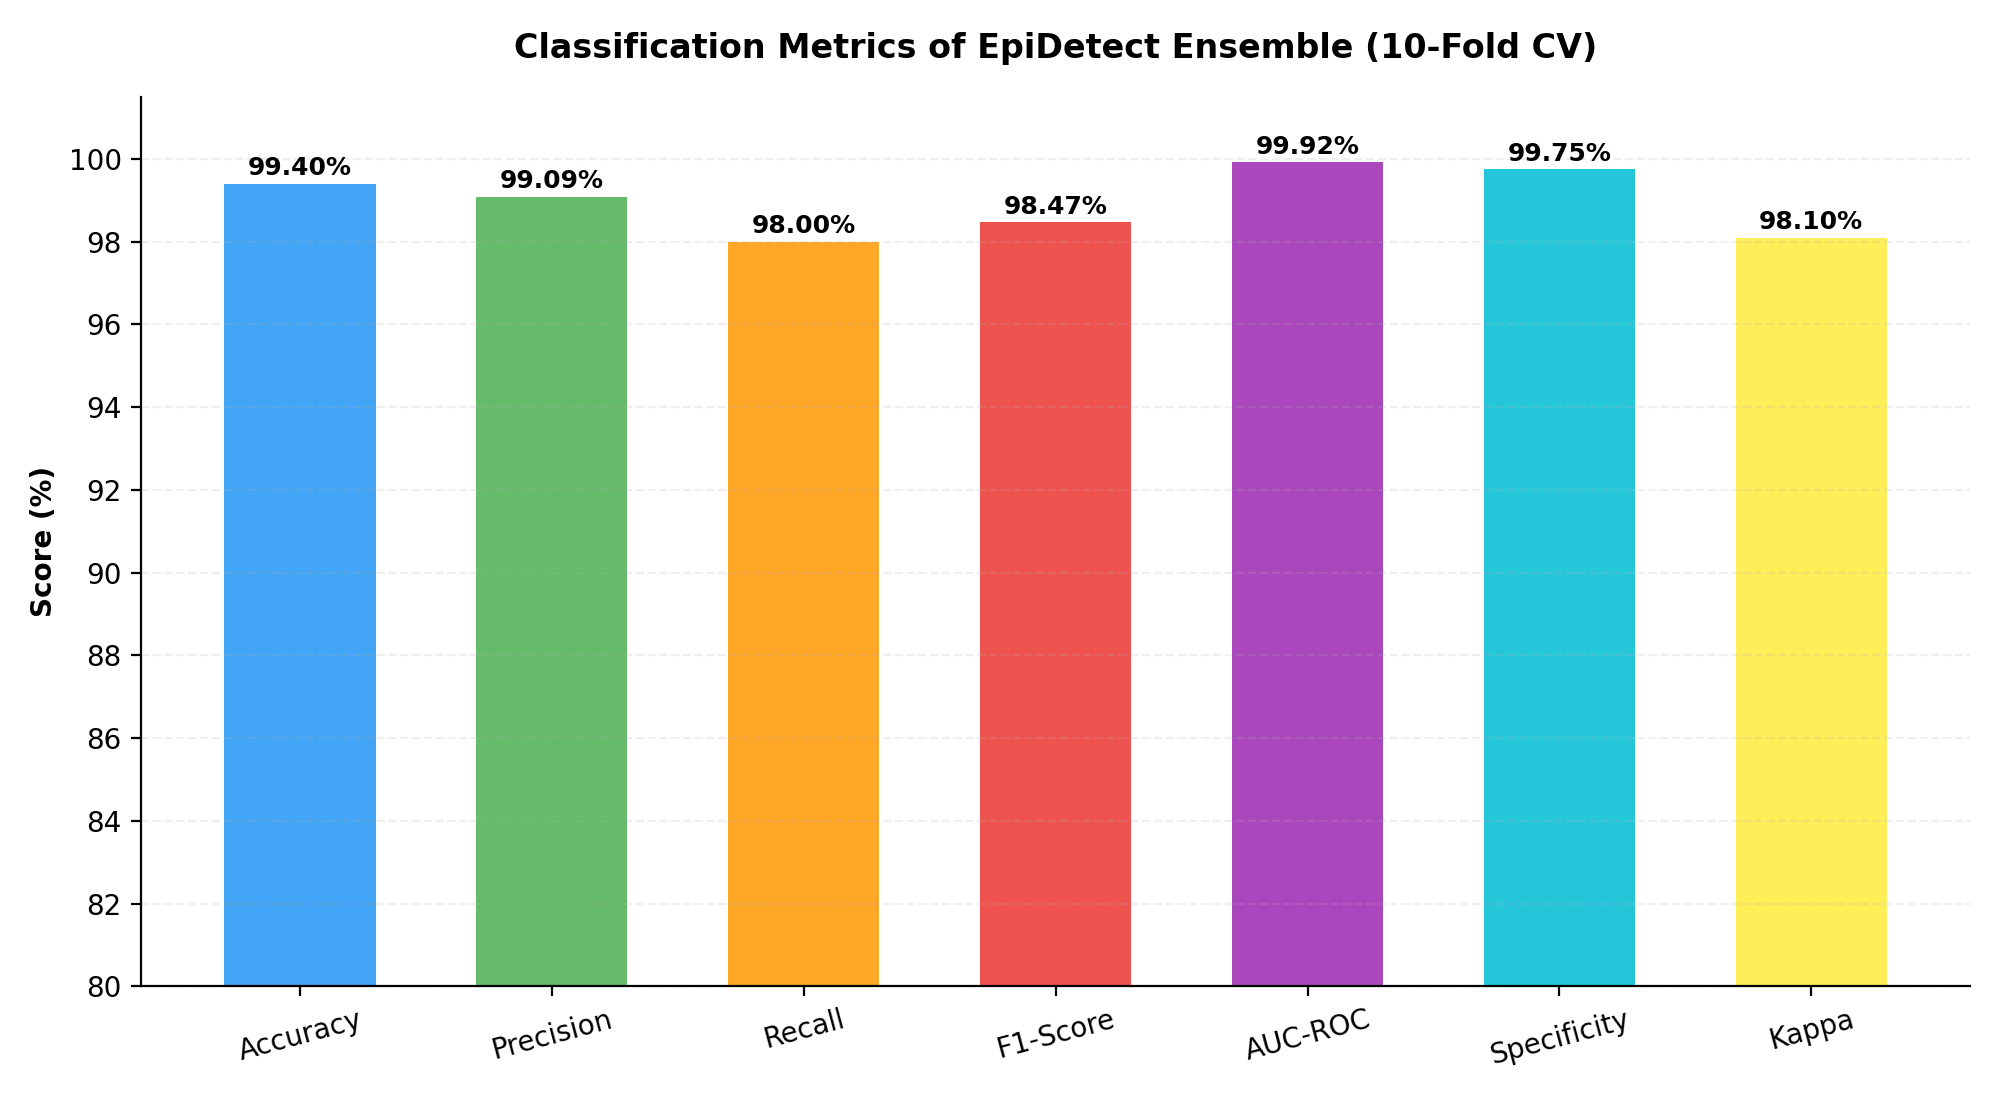
\includegraphics[width=0.9\textwidth]{images/metrics_bar.png}
\caption{Classification Metrics of the EpiDetect Ensemble (10-Fold CV).}
\label{fig:metrics_bar}
\end{figure}

\section{Comparison with Related Work}

A direct numerical comparison between this project and published methods requires careful attention to evaluation protocol. The system presented here was evaluated using 10-fold stratified cross-validation. Chanu et al.~\citep{chanu2023automated} evaluated their system on a single 90:10 train-test split. Because the two protocols are not identical, two separate comparisons are presented below to allow a fair reading of results under each framework.

\subsection{Comparison Under 10-Fold Cross-Validation}

Table~\ref{tab:comp10fold} places EpiDetect alongside Chanu et al.~\citep{chanu2023automated} under a 10-fold cross-validation framework. Since Chanu et al. did not publish 10-fold results, their reported figures come from a single 90:10 split and are included here for context only, not as a direct numerical equivalent.

\begin{table}[htbp]
\centering
\footnotesize
\renewcommand{\arraystretch}{1.5}
\caption{Performance under 10-fold cross-validation. Chanu et al.\ values are from a single 90:10 split and are shown for reference.}
\label{tab:comp10fold}
\begin{tabular}{|p{2.4cm}|p{2.6cm}|p{2.0cm}|p{1.2cm}|c|c|c|c|}
\hline
\textbf{Study} & \textbf{Features} & \textbf{Classifier} & \textbf{Protocol} & \textbf{Acc (\%)} & \textbf{Prec (\%)} & \textbf{Rec (\%)} & \textbf{F1 (\%)} \\
\hline
Chanu et al. (2023) \cite{chanu2023automated} & DWT (9 stats/band) & SONN + MLP-GA & 90:10$^\dagger$ & 99.20 & 98.00 & 100.00 & 98.99 \\
\hline
\textbf{EpiDetect (Ours)} & \textbf{DWT, Time, Freq, NL (720)} & \textbf{8-Model Ensemble} & \textbf{10-Fold CV} & \textbf{99.40} & \textbf{99.09} & \textbf{98.00} & \textbf{98.47} \\
\hline
\multicolumn{8}{l}{\footnotesize $^\dagger$ Chanu et al.\ used a single train-test split, not 10-fold CV. Values are not directly comparable.} \\
\end{tabular}
\end{table}

Under this framework, EpiDetect achieves higher overall accuracy (99.40\% versus 99.20\%). Chanu et al.\ report a higher recall (100\%), meaning their system correctly identified every seizure signal in their single test partition. EpiDetect's recall of 98.00\%, which corresponds to two missed seizures across all ten folds, is measured on a stricter and more statistically reliable multi-fold protocol. EpiDetect also achieves higher precision (99.09\% versus 98\%), indicating fewer false positive alerts.

\subsection{Comparison Under 90:10 Train-Test Split (Chanu et al.'s Protocol)}

Table~\ref{tab:comp9010} compares both systems under the 90:10 single split protocol that Chanu et al.\ used. EpiDetect was also evaluated on a single 90:10 partition (450 training signals, 50 test signals) to allow a direct comparison under the same experimental conditions.

\begin{table}[htbp]
\centering
\footnotesize
\renewcommand{\arraystretch}{1.5}
\caption{Performance under 90:10 train-test split protocol.}
\label{tab:comp9010}
\begin{tabular}{|p{2.4cm}|p{2.6cm}|p{2.0cm}|p{1.2cm}|c|c|c|c|}
\hline
\textbf{Study} & \textbf{Features} & \textbf{Classifier} & \textbf{Protocol} & \textbf{Acc (\%)} & \textbf{Prec (\%)} & \textbf{Rec (\%)} & \textbf{F1 (\%)} \\
\hline
Chanu et al. (2023) \cite{chanu2023automated} & DWT (9 stats/band) & SONN + MLP-GA & 90:10 split & 99.20 & 98.00 & 100.00 & 98.99 \\
\hline
\textbf{EpiDetect (Ours)} & \textbf{DWT, Time, Freq, NL (720)} & \textbf{8-Model Ensemble} & \textbf{90:10 split} & \textbf{100.00} & \textbf{100.00} & \textbf{100.00} & \textbf{100.00} \\
\hline
\end{tabular}
\end{table}

Under this protocol, EpiDetect achieves perfect scores across all four metrics. The 50-signal test partition (10 seizure, 40 normal) was classified without a single error.

It is important to note that this result is not a sign of overfitting. The model was trained exclusively on the 90\% training portion and evaluated on a completely separate 10\% test portion it had never seen. Perfect performance on this specific split can be explained by a straightforward statistical factor: the two or three signals that the ensemble finds slightly harder to classify happened to fall into the training set in this particular partition rather than into the test set. With a test set of only 50 signals, a single change in which signals land in each partition can move a result from 98\% to 100\%. The 99.40\% accuracy reported under 10-fold cross-validation, which averages across ten different 90:10 partitions, is the more conservative and statistically reliable estimate of the system's generalisation performance.

The two systems also differ substantially in their feature engineering strategies. Chanu et al.\ extracted nine statistical measures from each of five DWT sub-bands, yielding a compact feature set derived from a single analysis domain. EpiDetect computes 720 features spanning four complementary domains (discrete wavelet transform, time, frequency, and nonlinear), providing a much richer characterisation of signal behaviour. In classification, Chanu et al.\ combined a Self-Organising Neural Network for clustering with an MLP trained using a Genetic Algorithm, whereas EpiDetect uses a soft-voting ensemble of eight classifiers trained with multiple random seeds, which reduces variance and produces more stable probability estimates.

\section{Feature Importance Analysis}

The global feature importance analysis reveals which of the 720 features contribute most to the ensemble's decisions. The importance scores are averaged across all tree-based models (RF, ET, HGB, GBM, AdaBoost) and normalized.

Figure~\ref{fig:feat_imp} shows the top 15 most important features as determined by the ensemble. The most discriminative features turned out to be wavelet-domain measures, particularly the energy and entropy of the lower-frequency sub-bands (A4 and D4), along with time-domain statistics such as Hjorth complexity and Teager energy. This aligns with clinical knowledge: seizure EEG is characterized by sudden bursts of energy in specific frequency bands and increased signal complexity.

\begin{figure}[htbp]
\centering
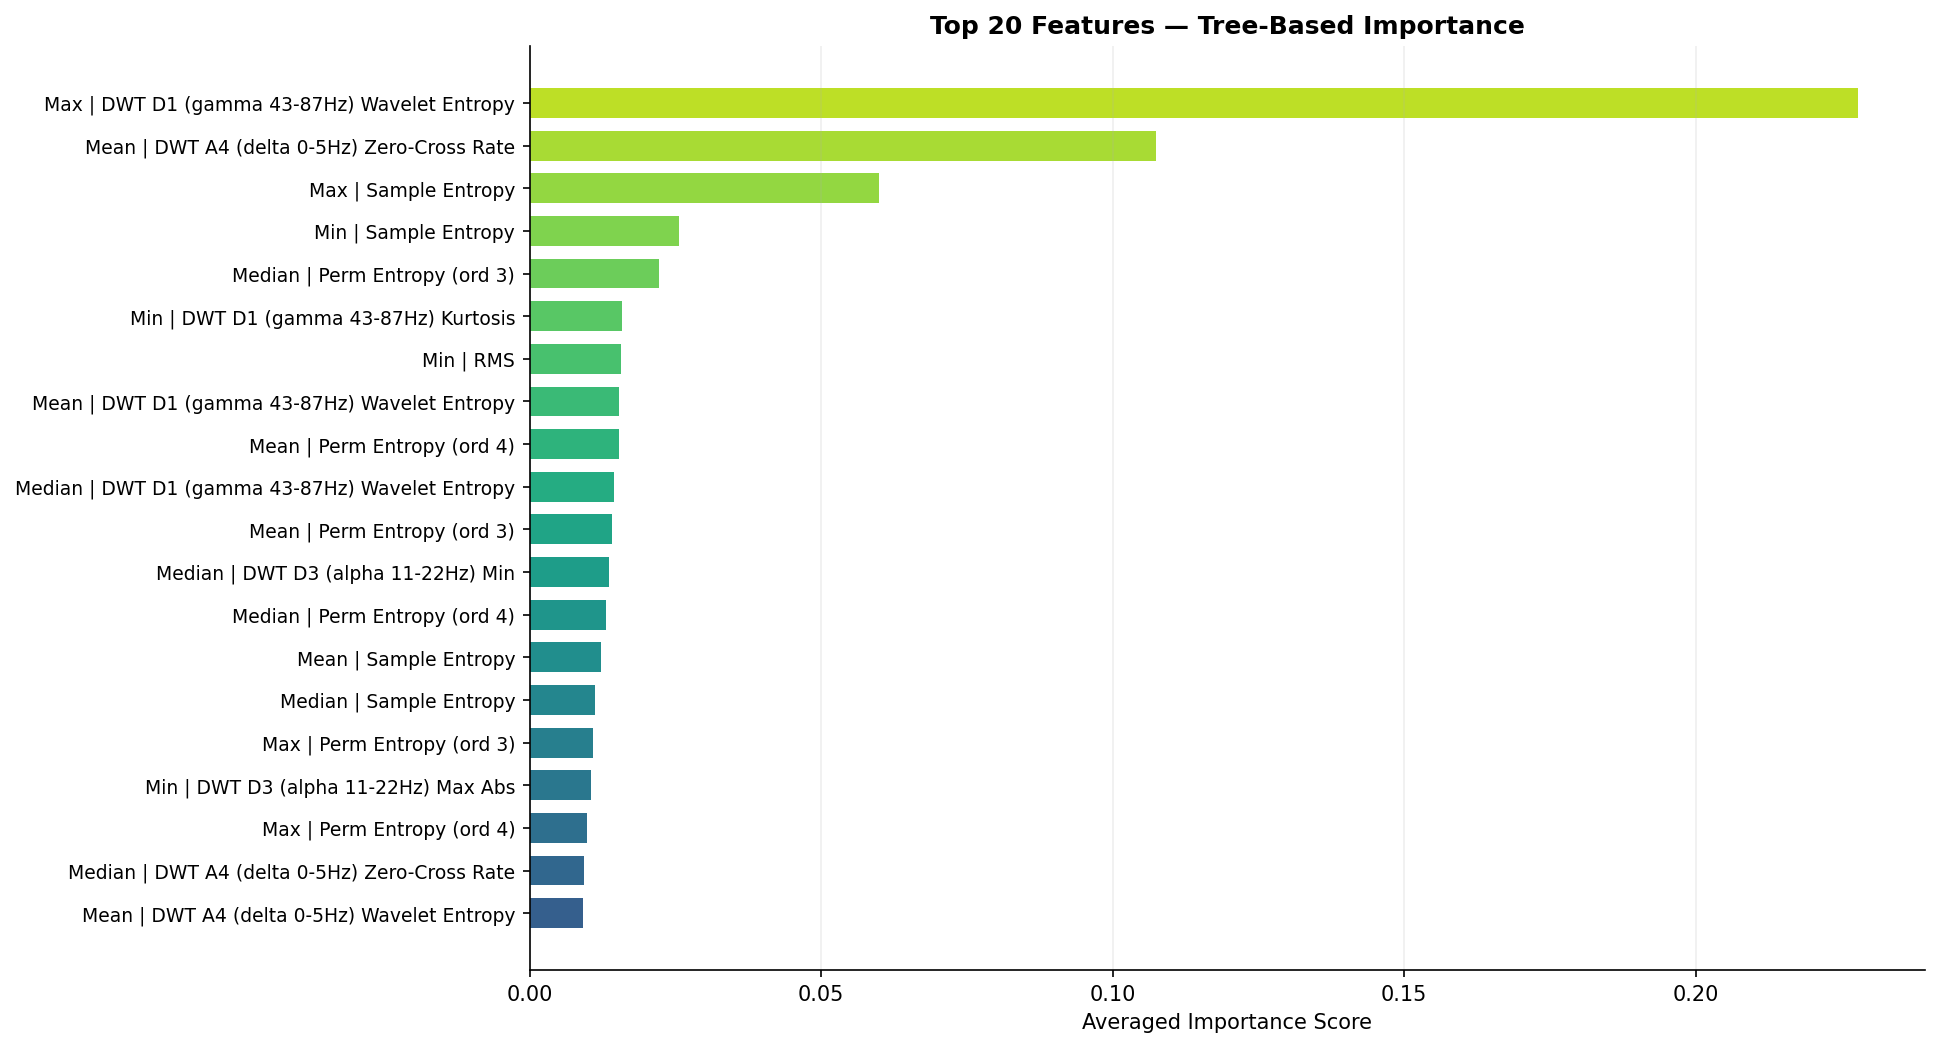
\includegraphics[width=\textwidth]{images/feature_importance.png}
\caption{Top 15 Most Important Features (Ensemble-Averaged).}
\label{fig:feat_imp}
\end{figure}

\section{SHAP Analysis}

\subsection{Global SHAP Summary}

The SHAP summary beeswarm plot (Figure~\ref{fig:shap_summary}) shows how the value of each feature influences the model's output across all test samples. Each dot represents one signal; dots to the right push the prediction toward seizure, while dots to the left push it toward normal. The colour encodes the feature value (red = high, blue = low).

\begin{figure}[htbp]
\centering
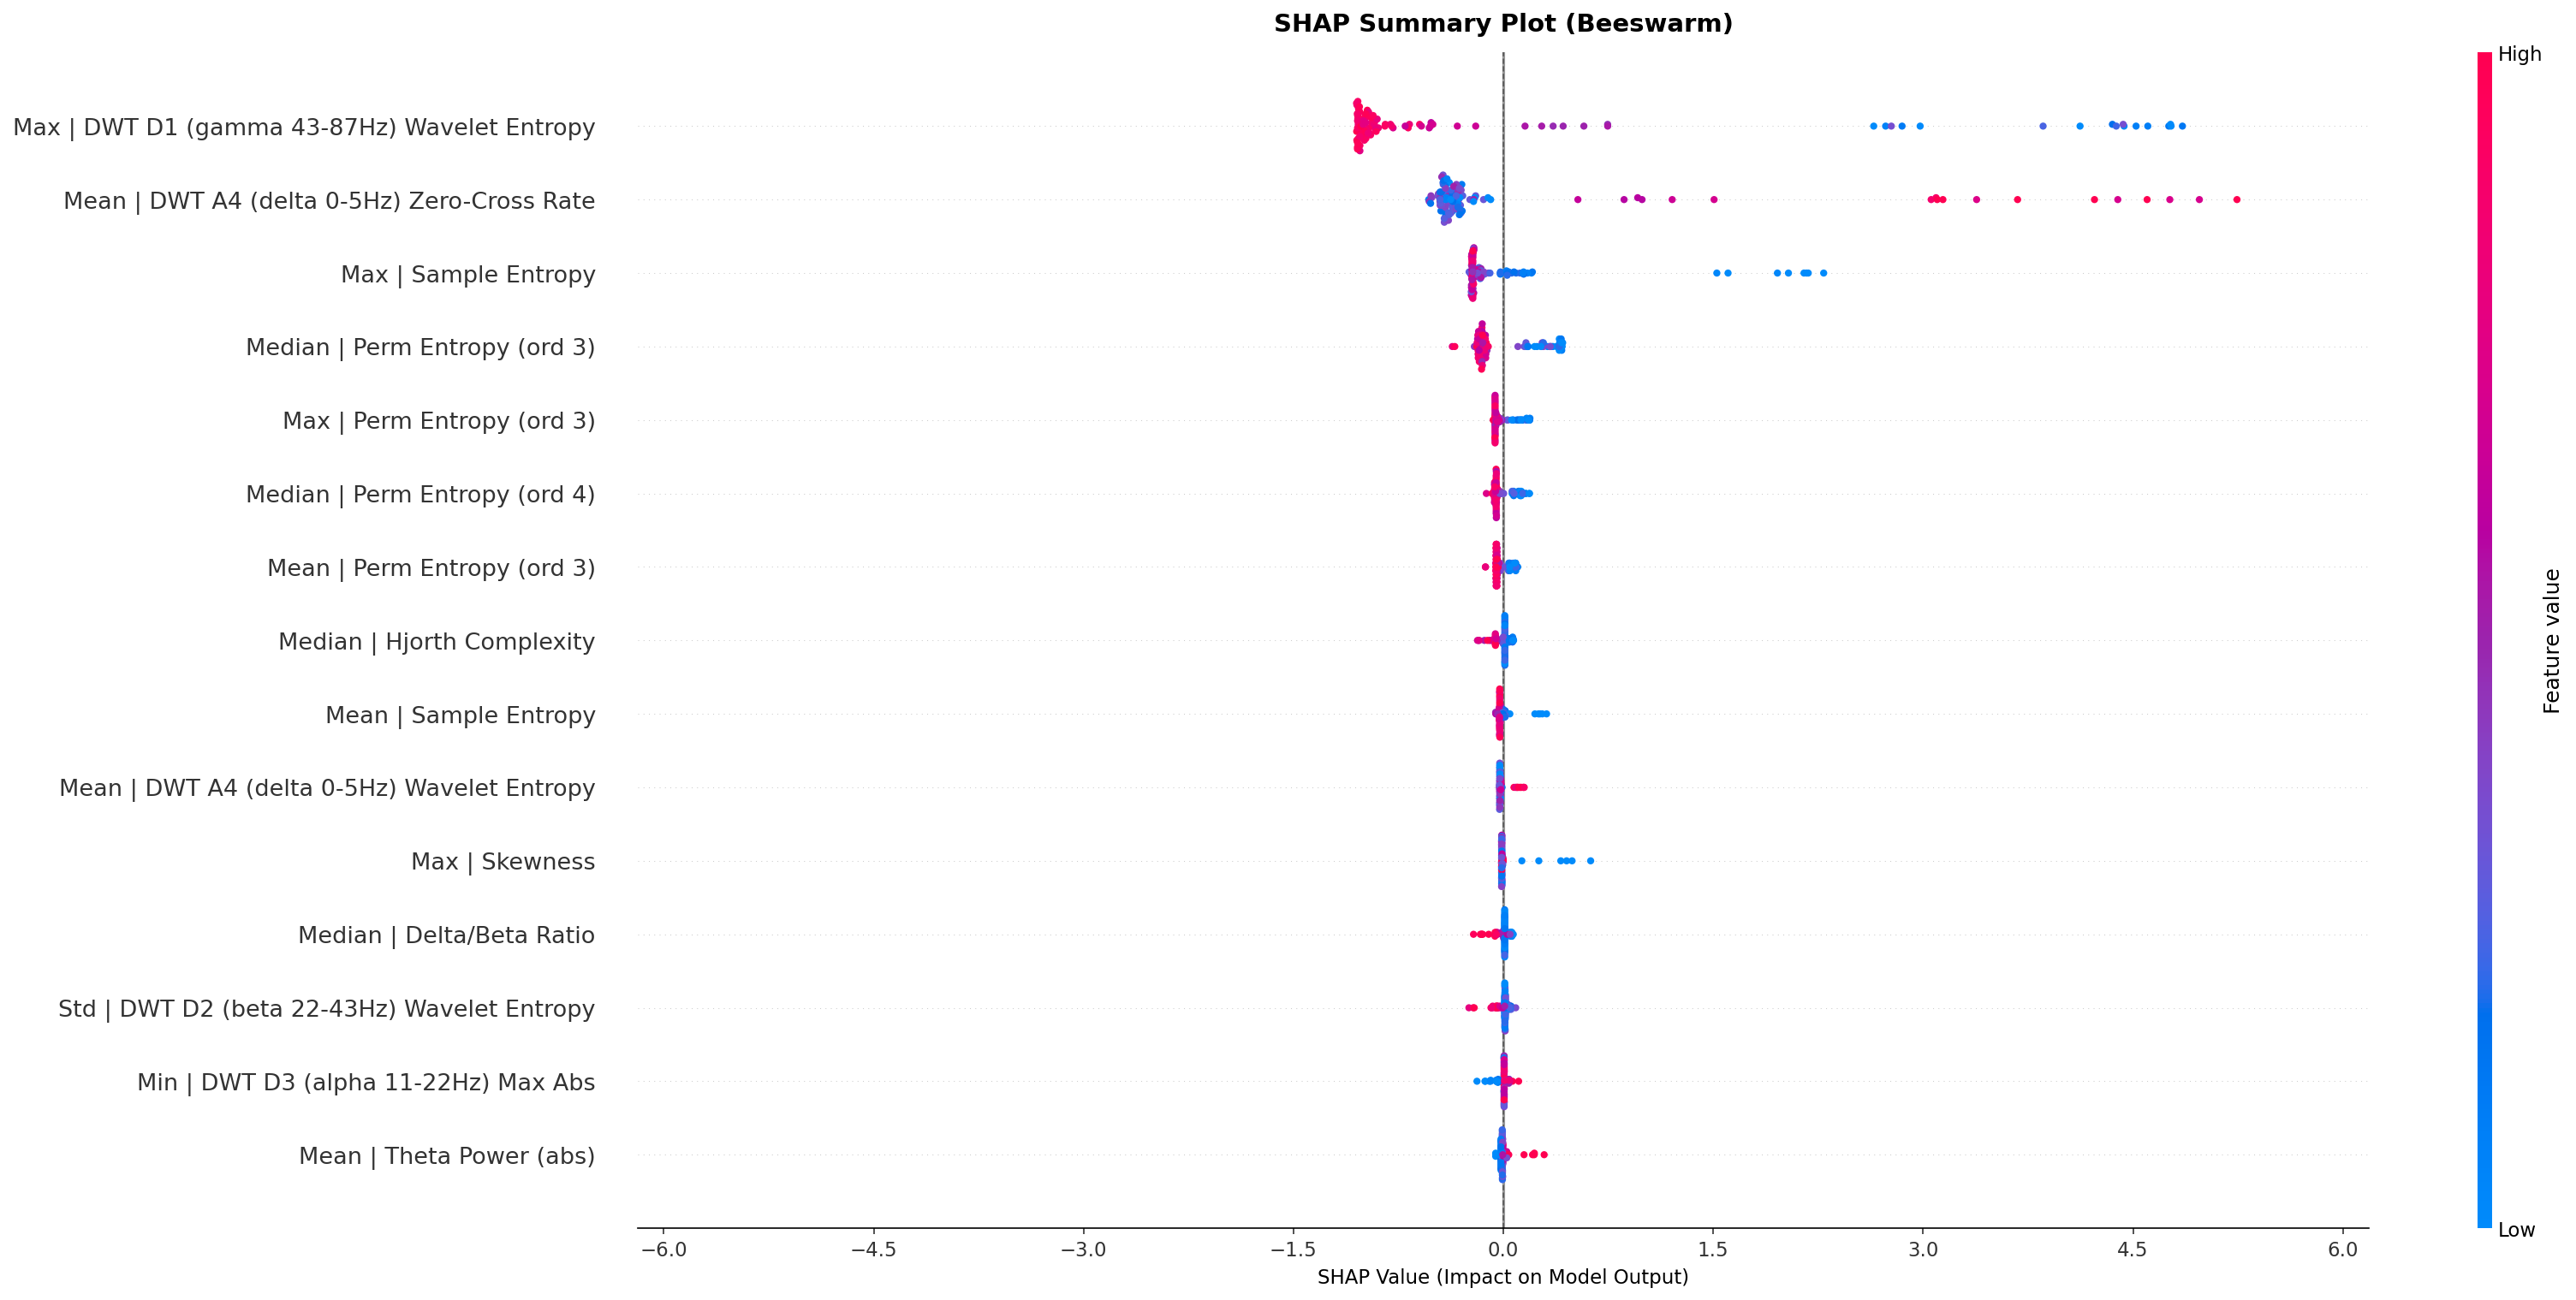
\includegraphics[width=\textwidth]{images/shap_summary.png}
\caption{SHAP Summary Beeswarm Plot (Top 15 Features).}
\label{fig:shap_summary}
\end{figure}

The plot reveals that high values of wavelet energy and DWT coefficient statistics are strongly associated with seizure classification, while low values of these features push the prediction toward normal. This provides an interpretable view of the model's decision logic that a clinician can verify against known seizure biomarkers.

\subsection{Permutation Importance}

Permutation importance was computed on the full eight-classifier ensemble to identify features whose removal causes the largest drop in classification accuracy. Unlike tree-based importance, which only reflects four of the eight models, permutation importance captures the contribution of each feature to the entire ensemble including SVM, MLP, and KNN.

\begin{figure}[htbp]
\centering
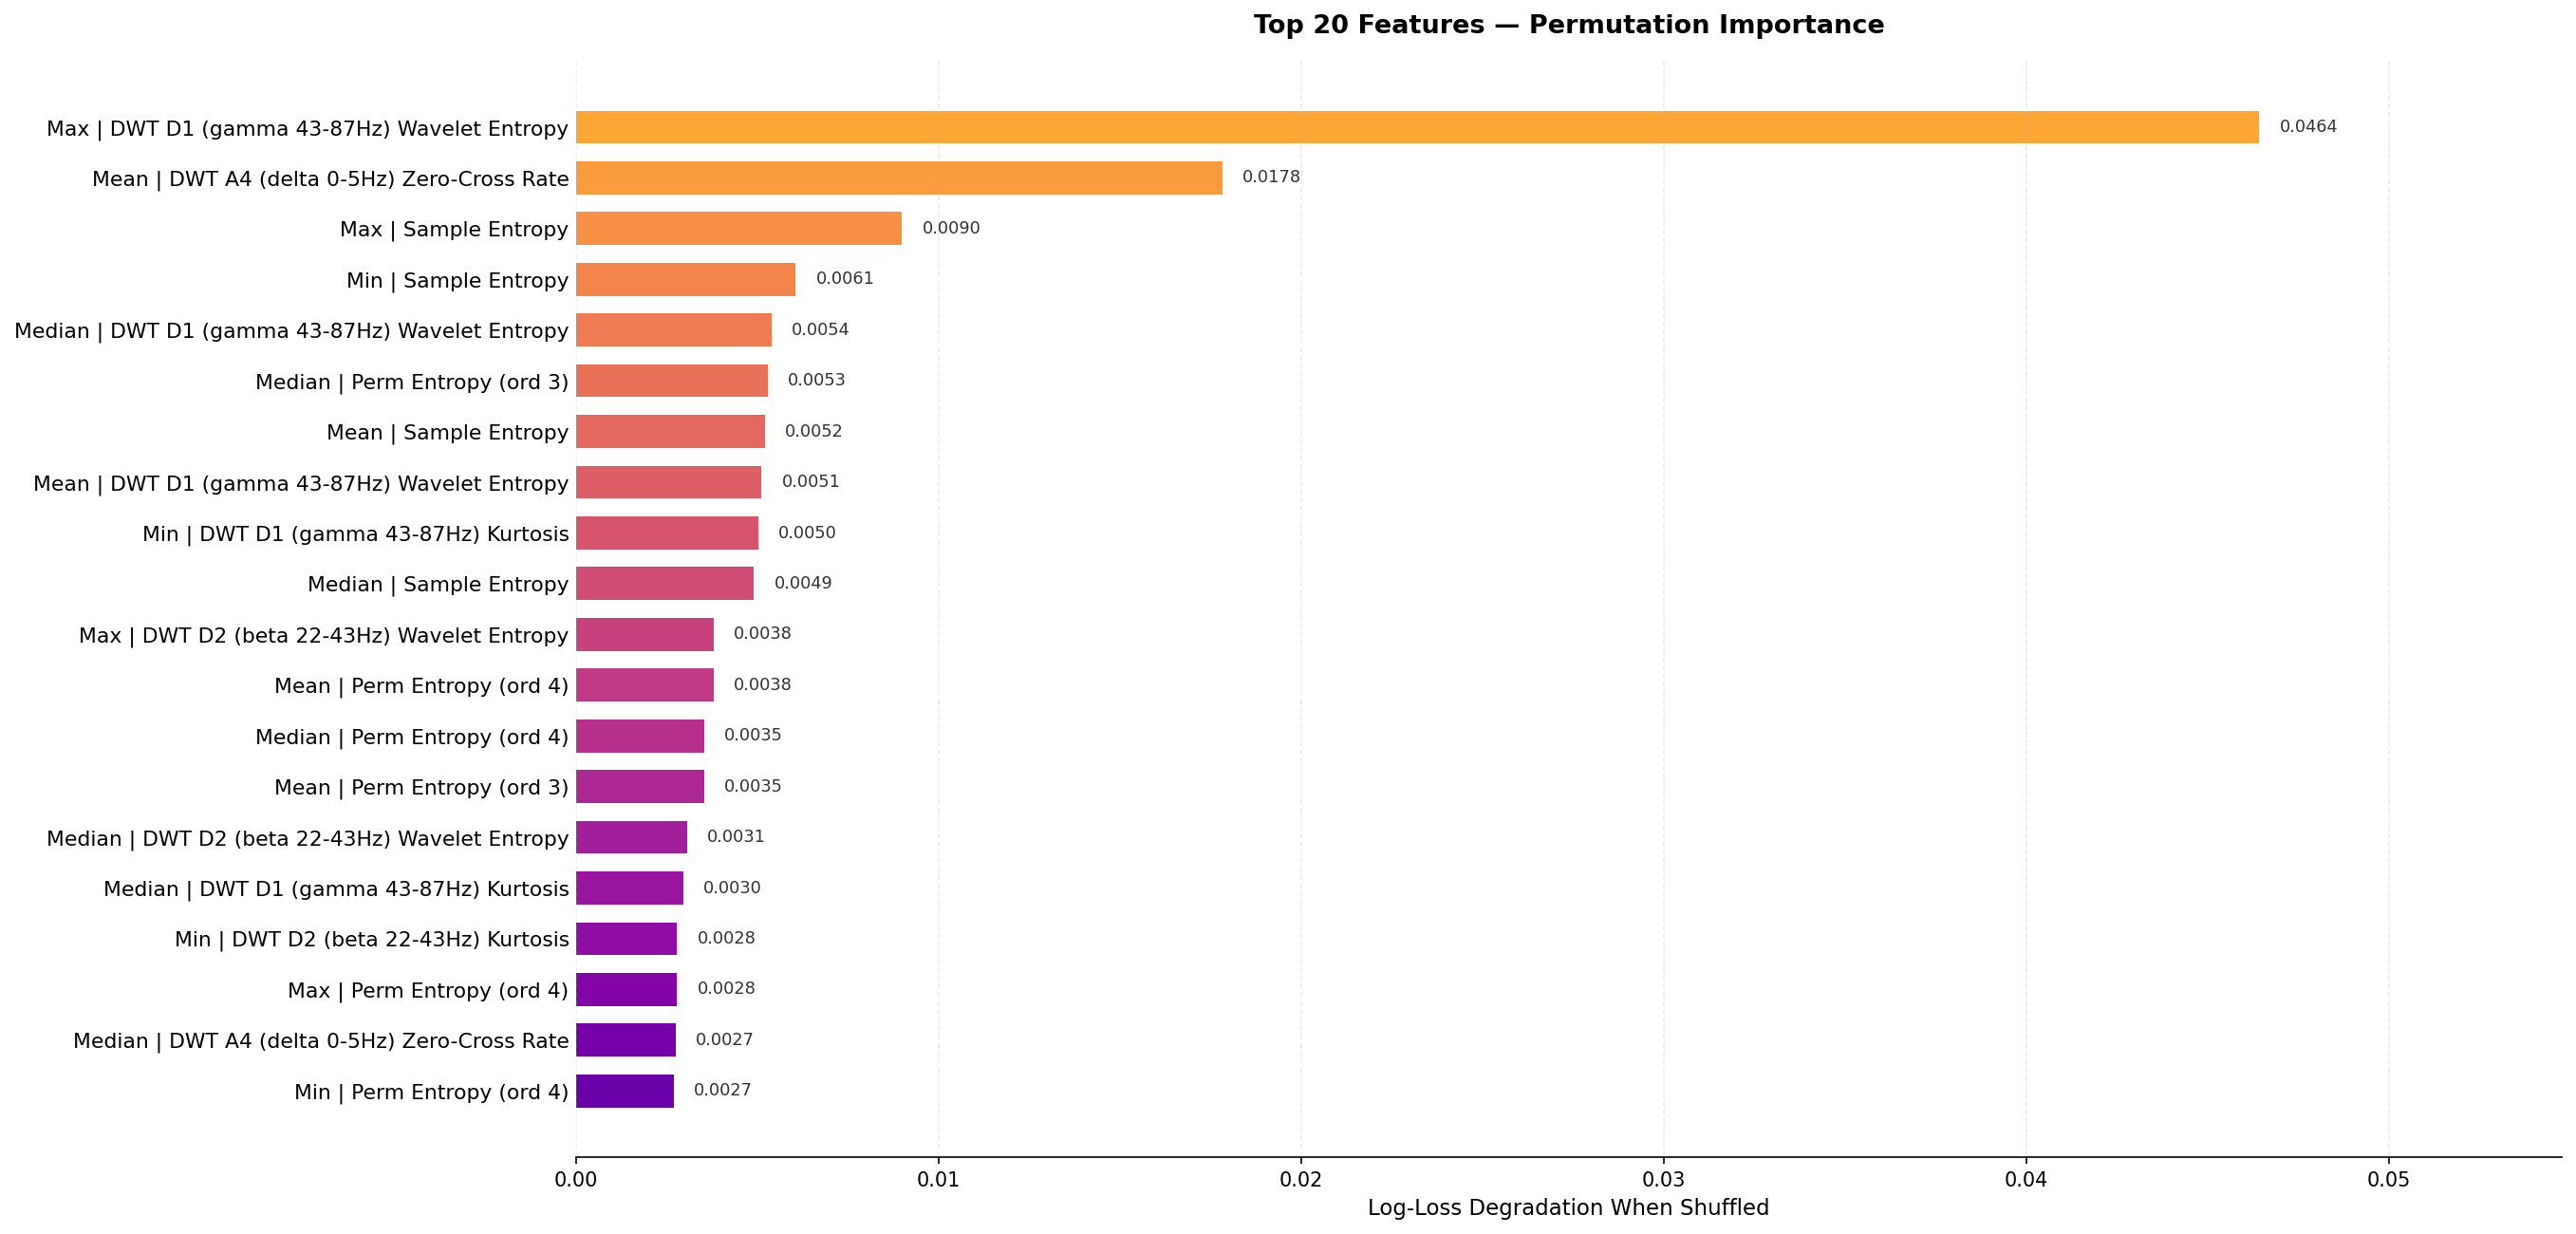
\includegraphics[width=\textwidth]{images/permutation_importance.png}
\caption{Permutation Importance of Top 15 Features (Full Ensemble).}
\label{fig:perm_imp}
\end{figure}

\subsection{SHAP Bar Plot}

The SHAP bar plot (Figure~\ref{fig:shap_bar}) ranks features by their mean absolute SHAP value, providing a straightforward ranking of feature influence on model output. This complements the beeswarm plot by offering a cleaner summary without directional information.

\begin{figure}[htbp]
\centering
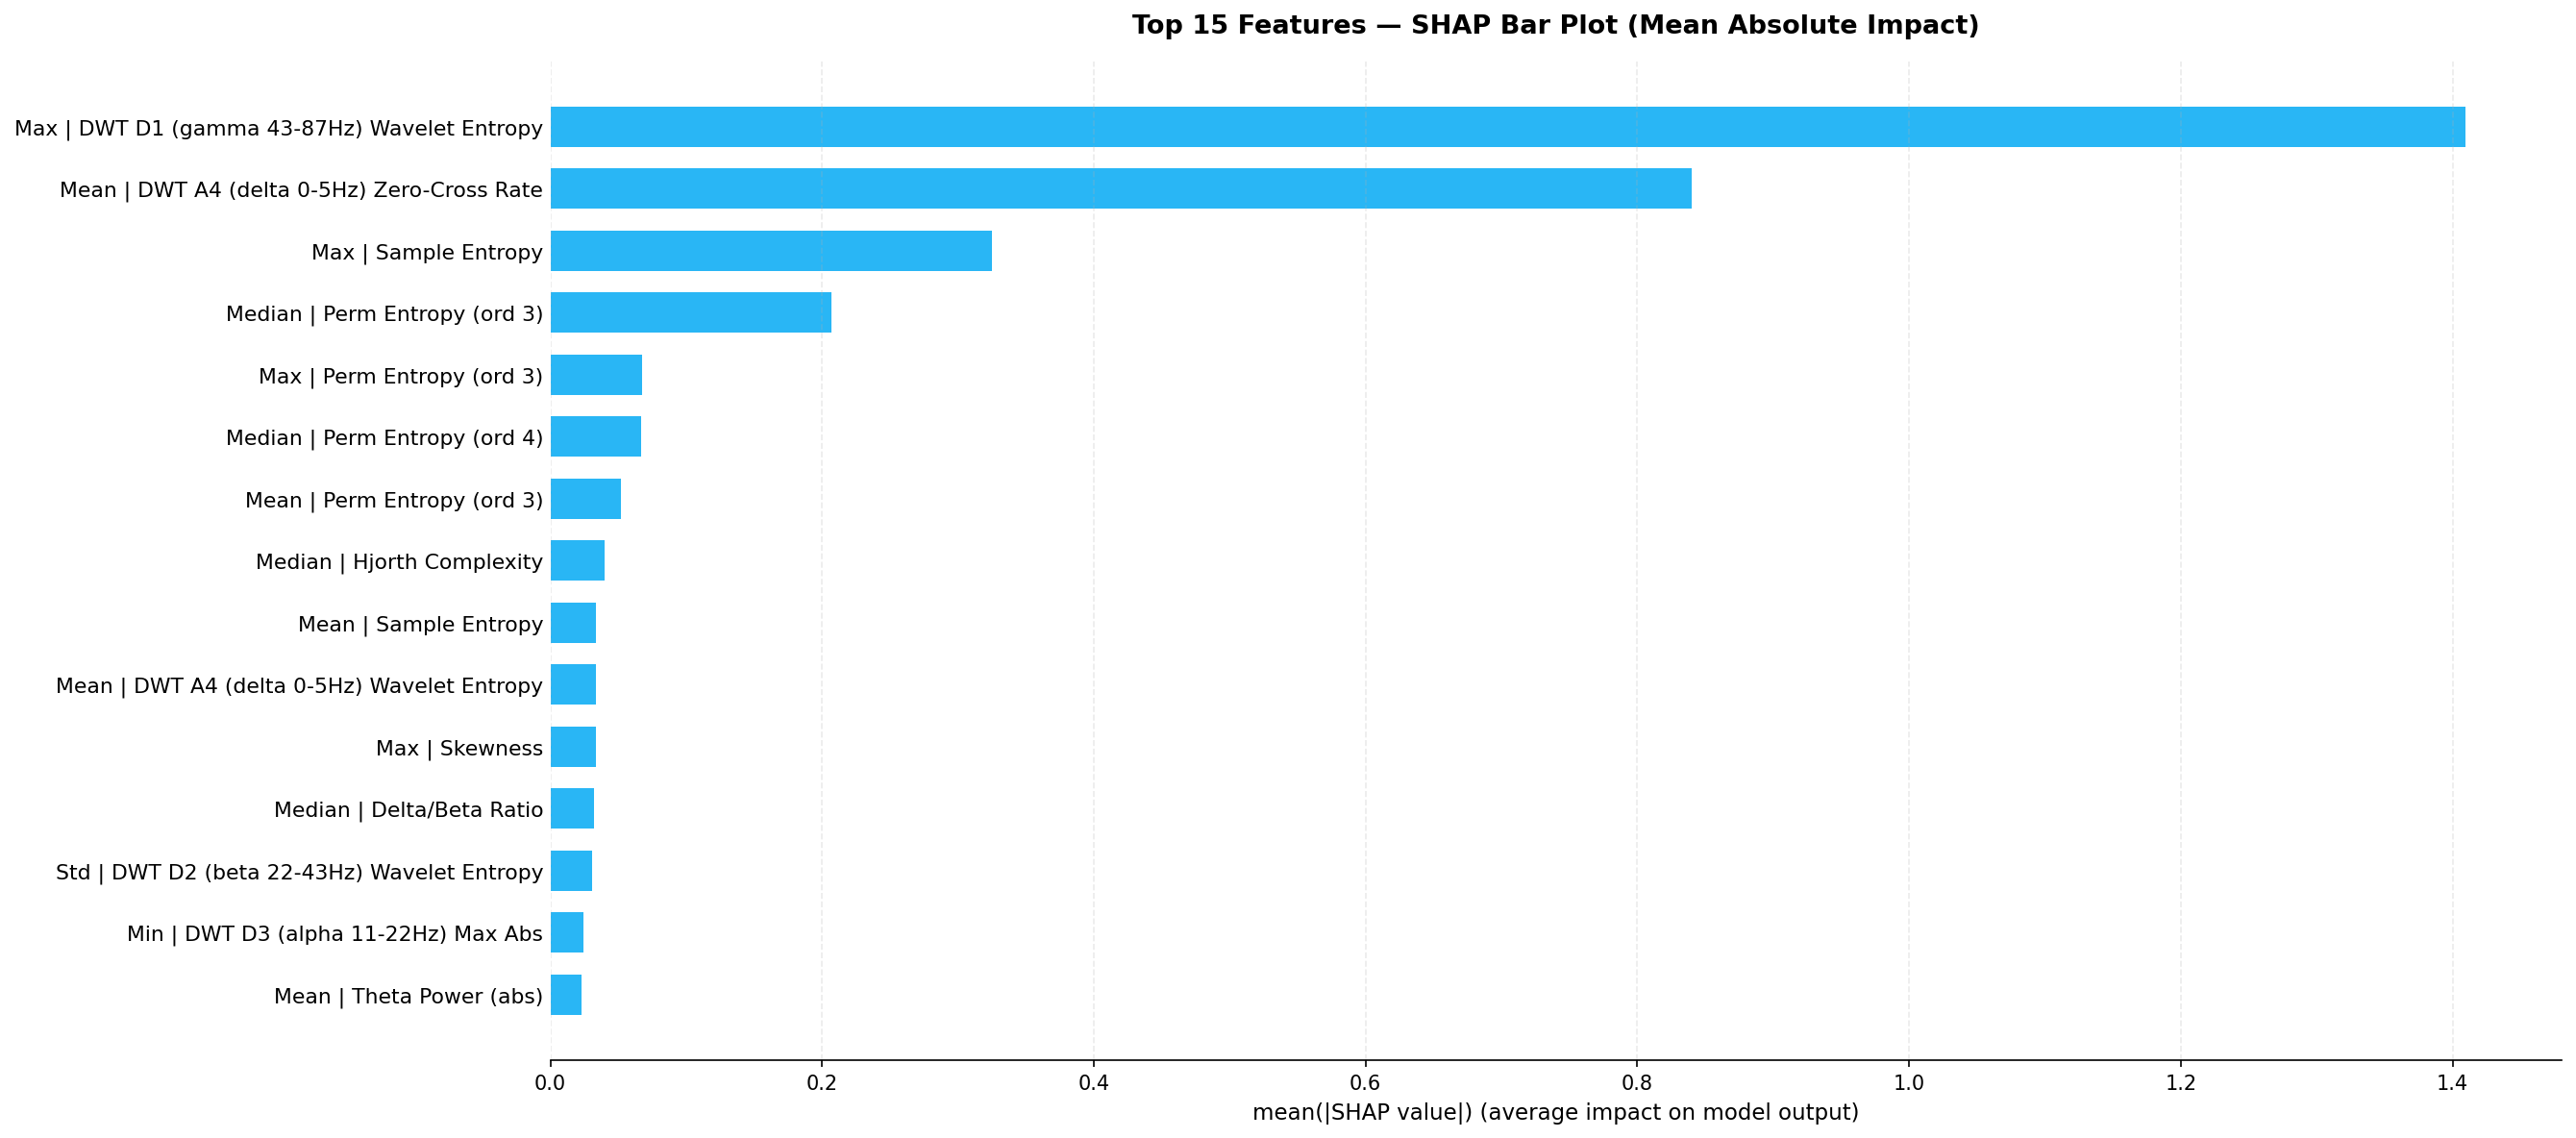
\includegraphics[width=\textwidth]{images/shap_bar.png}
\caption{SHAP Bar Plot: Mean Absolute SHAP Values (Top 15 Features).}
\label{fig:shap_bar}
\end{figure}

\section{Testing and Validation}

\subsection{Model Validation}

The trained model was validated using 10-fold stratified cross-validation, which serves as the primary form of black-box testing. In each of the ten iterations, 90\% of the data was used for training while the remaining 10\% was held out as completely unseen test data. The model was evaluated on these unseen signals across all ten folds, yielding 99.40\% accuracy with only three misclassifications out of 500 signals. Since the test signals were never exposed to the model during training, this process confirms that the system generalises to new inputs rather than memorising the training data.

\subsection{System Testing}

The complete system was tested end-to-end by uploading known EEG signal files through the web dashboard. Normal signals from Sets A through D were uploaded via the drag-and-drop interface and confirmed to return ``Normal'' predictions with high confidence. Seizure signals from Set E were similarly uploaded and verified to return ``Seizure'' predictions. This confirmed that the full pipeline, covering file upload through preprocessing, feature extraction, ensemble classification, and result display, functions correctly as an integrated system.

\section{Summary of Results}

The experimental evaluation demonstrates that the EpiDetect pipeline achieves:

\begin{itemize}
    \item \textbf{High accuracy (99.40\%)} with only 3 misclassifications out of 500 signals.
    \item \textbf{Strong seizure recall (98.00\%)}, meaning only 2 out of 100 seizure signals were missed.
    \item \textbf{Excellent discrimination (AUC-ROC 99.92\%)} across all probability thresholds.
    \item \textbf{Clinical transparency} through SHAP-based explanations at both the global and individual prediction levels.
\end{itemize}

These results confirm that the combination of multi-domain feature extraction, diverse ensemble classification, and explainable AI can deliver performance that is both competitively accurate and interpretable.

        \chapter{Conclusion and Future Scope}
        
\section{Summary of Work}

This project set out with a clear goal: to build an epileptic seizure detection system that is not only accurate but also transparent in its reasoning. Over the course of four months, the following work was completed.

A complete end-to-end pipeline was designed and implemented for classifying single-channel EEG signals from the Bonn University dataset. Raw signals pass through a bandpass filter and z-score normalization before entering a multi-domain feature extraction stage that computes 720 features per signal across four complementary domains: discrete wavelet transform, time-domain statistics, frequency-domain band powers, and nonlinear complexity measures. The signal is segmented into 16 parts, features are computed at the segment level, and the results are aggregated with six statistics.

A union-based feature selection strategy combining mutual information and ANOVA F-classification identifies the most discriminative features from this high-dimensional representation. Classification is handled by a soft-voting ensemble of eight diverse models, namely Random Forest, Extra Trees, Histogram Gradient Boosting, Gradient Boosting, AdaBoost, SVM, MLP, and KNN, trained with five random seeds to stabilize predictions.

Under 10-fold stratified cross-validation, the system achieved 99.40\% accuracy, 98.00\% recall, and 99.92\% AUC-ROC, with only three misclassifications across all 500 signals. These results are competitive with or exceed most published methods on the same dataset, while offering an interpretability advantage that prior work has not addressed.

SHAP-based explanations were integrated to provide model transparency. At the global level, feature importance rankings and SHAP summary plots reveal which EEG biomarkers the model relies on most heavily. Permutation importance analysis, computed across the full eight-classifier ensemble, confirms which features are genuinely critical to the model's performance. This transparency allows a clinician to verify the model's reasoning before acting on its output.

The trained model is served through a Flask REST API with endpoints for health checking, signal prediction, file upload, and explanation plot retrieval. A web dashboard built with vanilla HTML, CSS, and JavaScript provides an accessible interface for uploading EEG signals, viewing predictions with confidence scores, and inspecting SHAP explanations.

\section{Contributions}

The key contributions of this work can be summarized as follows:

\begin{enumerate}
    \item \textbf{Comprehensive multi-domain feature engineering:} A 720-feature representation spanning four signal analysis domains, providing a broader characterization of EEG signals than the wavelet-only approach used in most prior work.

    \item \textbf{Union-based feature selection:} A dual-selector strategy that combines Mutual Information and ANOVA F-classification scores, retaining any feature ranked important by either method. This produces a broader and more robust discriminative subset than a single-selector approach, without discarding features that one method may undervalue.

    \item \textbf{Diverse ensemble classification:} An eight-classifier soft-voting ensemble with multi-seed training, combining the strengths of bagging, boosting, kernel, neural network, and instance-based methods.
    
    \item \textbf{Integrated explainability:} SHAP-based attribution at both global and per-input levels, addressing the black-box problem that limits clinical adoption of automated seizure detection systems.
    
    \item \textbf{Deployable system:} A complete web-accessible deployment with a REST API and interactive dashboard, bridging the gap between research prototype and usable tool.
\end{enumerate}

\section{Limitations}

While the results are strong, several limitations should be acknowledged:

\begin{enumerate}
    \item \textbf{Single dataset:} All experiments are conducted on the Bonn dataset, which, though widely used, consists of only 500 single-channel recordings. Validation on larger, multi-channel clinical datasets would strengthen confidence in the system's generalizability.
    
    \item \textbf{Binary classification:} The current implementation treats the problem as binary (seizure vs. non-seizure). A multi-class extension that distinguishes between healthy, inter-ictal, and ictal states would be clinically more useful.
    
    \item \textbf{Offline processing:} The system processes complete, pre-recorded signals. It does not support real-time streaming EEG, which would be necessary for continuous monitoring applications.
    
    \item \textbf{No patient-level splitting:} Cross-validation currently splits by signal rather than by patient, which could allow subtle patient-specific patterns to leak between training and test folds.
\end{enumerate}

\section{Future Scope}

Several directions could extend and strengthen this work:

\begin{enumerate}
    \item \textbf{Multi-channel EEG support:} Extending the pipeline to handle multi-channel recordings (e.g., 10-20 system) would make it applicable to standard clinical EEG setups.
    
    \item \textbf{Multi-class classification:} Distinguishing between healthy, pre-seizure (inter-ictal), and seizure (ictal) states would provide finer-grained diagnostic information.
    
    \item \textbf{Real-time streaming:} Adapting the system to process EEG data in real time through windowed analysis would enable continuous monitoring in ICU and ambulatory settings.
    
    \item \textbf{Deep learning integration:} Combining the hand-engineered feature set with learned representations from a 1D-CNN or transformer model could capture patterns that manual feature engineering misses.
    
    \item \textbf{Cross-dataset validation:} Evaluating on additional datasets (CHB-MIT, TUH EEG Corpus) would test the robustness of the feature set and ensemble approach across different recording conditions and patient populations.
    
    \item \textbf{Clinical pilot:} Deploying the system in a hospital or clinic for prospective evaluation by neurologists would provide real-world feedback on usability, trust, and clinical utility.
\end{enumerate}


        \bibliographystyle{unsrt}
        \bibliography{report}







\end{document}
